%%%%%%%% ICML 2025 EXAMPLE LATEX SUBMISSION FILE %%%%%%%%%%%%%%%%%

\documentclass{article}
\usepackage[T1]{fontenc}
\usepackage{inconsolata}

\usepackage{enumitem}
\usepackage{hyperref}


% Attempt to make hyperref and algorithmic work together better:
\newcommand{\theHalgorithm}{\arabic{algorithm}}

% Use the following line for the initial blind version submitted for review:
\usepackage{icml2025_anon} %% DON'T USE FOR FINAL PAPER

% If accepted, instead use the following line for the camera-ready submission:
% \usepackage[accepted]{icml2025}

% For theorems and such
\newcommand{\xhdr}[1]{{\noindent\bfseries #1}.}

\usepackage{amsmath}
\usepackage{amssymb}
\usepackage{mathtools}
\usepackage{amsthm}
\usepackage{graphicx}
\usepackage{booktabs}
\usepackage{colortbl}
\usepackage{makecell}
\usepackage{caption}
\usepackage{multirow}
\usepackage{listings}
\usepackage{cuted}
\usepackage{multicol}
\usepackage{titling}
\usepackage{manyfoot}
\usepackage{verbatim}
\usepackage{xspace}
\usepackage{marginnote}
\usepackage{xcolor}
% if you use cleveref..
\usepackage[capitalize,noabbrev]{cleveref}

\usepackage{tikz}
\newcommand*\circled[1]{\tikz[baseline=(char.base)]{
            \node[shape=circle,draw,inner sep=0.5pt] (char) {#1};}}

%%%%%%%%%%%%%%%%%%%%%%%%%%%%%%%%
% THEOREMS
%%%%%%%%%%%%%%%%%%%%%%%%%%%%%%%%
\theoremstyle{plain}
\newtheorem{theorem}{Theorem}[section]
\newtheorem{proposition}[theorem]{Proposition}
\newtheorem{lemma}[theorem]{Lemma}
\newtheorem{corollary}[theorem]{Corollary}
\theoremstyle{definition}
\newtheorem{definition}[theorem]{Definition}
\newtheorem{assumption}[theorem]{Assumption}
\theoremstyle{remark}
\newtheorem{remark}[theorem]{Remark}
\usepackage{tabularx}
\usepackage{quoting}
\newenvironment{ex}[1]
 {%
  \quoting[leftmargin=0.1cm,rightmargin=0.1cm]%
  \noindent\textcolor{blue!75}{} \itshape\ignorespaces
 }
 {\endquoting}
\newcommand{\numturker}{201}
 \newcommand{\realsatisfy}{95.9\%\xspace}
 \newcommand{\realsatisfyimprov}{17.6\%\xspace}
 \newcommand{\realtimeimprov}{10.4\%\xspace}

 
\newcommand{\taskimprov}{18.5\%\xspace}
\newcommand{\itrimprov}{46.3\%\xspace}
\newcommand{\efficiencyimprov}{13.3\%\xspace}
\newcommand{\ie}{\textit{i.e., }}
\newcommand{\eg}{\textit{e.g., }}
\newcommand{\etal}{\textit{et al.}}
\newcommand{\st}{\textit{s.t. }}
\newcommand{\etc}{\textit{etc.}}
\newcommand{\wrt}{\textit{w.r.t. }}
\newcommand{\cf}{\textit{cf. }}
\newcommand{\aka}{\textit{aka. }}

% Customize monospaced font here. zi4 looks professional.
\renewcommand{\ttdefault}{zi4}

%\newcommand{\mathc }{\texttt{MATH-Chat} } 
%\newcommand{\mathct}{\texttt{MATH-Chat}} 
%\newcommand{\ambcoqa }{\texttt{Abg-CoQA} } 
%\newcommand{\ambcoqat}{\texttt{Abg-CoQa}} 
%\newcommand{\code }{\texttt{BigCodeBench-Chat} } 
%\newcommand{\codet}{\texttt{BigCodeBench-Chat}} 
%\newcommand{\doc }{\texttt{MediumDocEdit-Chat} } 
%\newcommand{\doct}{\texttt{MediumDocEdit-Chat}} 
%\newcommand{\llama}{\texttt{Meta-Llama-3.1-8B-Instruct }}
%\newcommand{\ourst}{\textsc{MR}} 
%\newcommand{\ours}{\textsc{MR }}
%\newcommand{\objectt}{interactive LLM}
%\newcommand{\object}{interactive LLM }
%\newcommand{\Objectt}{Interactive LLM}
%\newcommand{\Object}{Interactive LLM }
%\newcommand{\Objectst}{Interactive LLMs}
%\newcommand{\Objects}{Interactive LLMs }
%\newcommand{\objectst}{interactive LLMs}
%\newcommand{\objects}{interactive LLMs }

\renewcommand{\thefootnote}{\fnsymbol{footnote}}
% Please check this works, but \xspace should solve the spacing issues (the t versions could be removed).
\newcommand{\mathc}{\texttt{MATH-Chat}\xspace} 
\newcommand{\mathct}{\texttt{MATH-Chat}\xspace} 
\newcommand{\ambcoqa}{\texttt{Abg-CoQA}\xspace} 
\newcommand{\ambcoqat}{\texttt{Abg-CoQa}\xspace} 
\newcommand{\code}{\texttt{BigCodeBench-Chat}\xspace} 
\newcommand{\codet}{\texttt{BigCodeBench-Chat}\xspace} 
\newcommand{\doc}{\texttt{MediumDocEdit-Chat}\xspace} 
\newcommand{\doct}{\texttt{MediumDocEdit-Chat}\xspace} 
\newcommand{\llama}{Llama-3.1-8B\xspace}
\newcommand{\ourst}{\textsc{MR}\xspace} 
\newcommand{\ours}{\textsc{MR}\xspace}
% \newcommand{\objectt}{interactive LLM\xspace}
% \newcommand{\object}{interactive LLM\xspace}
% \newcommand{\Objectt}{Interactive LLM\xspace}
% \newcommand{\Object}{Interactive LLM\xspace}
% \newcommand{\Objectst}{Interactive LLMs\xspace}
% \newcommand{\Objects}{Interactive LLMs\xspace}
% \newcommand{\objectst}{interactive LLMs\xspace}
% \newcommand{\objects}{interactive LLMs\xspace}

\newcommand{\name}{\textsc{CollabLLM}\xspace}
\newcommand{\namewithspace}{\textsc{Collab LLM}\xspace}
\newcommand{\objectt}{collaborative LLM\xspace}
\newcommand{\object}{collaborative LLM\xspace}
\newcommand{\Objectt}{Collaborative LLM\xspace}
\newcommand{\Object}{Collaborative LLM\xspace}
\newcommand{\Objectst}{Collaborative LLMs\xspace}
\newcommand{\Objects}{Collaborative LLMs\xspace}
\newcommand{\objectst}{collaborative LLMs\xspace}
\newcommand{\objects}{collaborative LLMs\xspace}
\usepackage{inconsolata} % Import modern font package
\lstset{
  basicstyle=\fontfamily{pcr}\selectfont\itshape\small, % Monospace + Italic + Small font
  frame=tb,                   
  breaklines=true,             
  breakatwhitespace=false,     
  linewidth=\linewidth,        
  numbers=left,                
  numberstyle=\tiny\color{gray}, 
  xleftmargin=10pt,            
  framexleftmargin=10pt,       
  tabsize=4,                   
  showstringspaces=false,      
  keywordstyle=\color{blue}\bfseries,  
  commentstyle=\color{gray},   
  stringstyle=\color{red},     
  aboveskip=10pt,              
  belowskip=10pt               
}
\usepackage{pifont}
\usepackage{xcolor}
% Changes globally:
\setlist[itemize]{leftmargin=10pt, itemsep=0pt, topsep=0pt, parsep=0pt}

%\newcommand{\TODO}[2]{\textcolor{red}{\textbf{TODO (#1)}: \textit{#2}}}
%\newcommand{\jure}[1]{\textcolor{red}{\textbf{Jure}: \textit{#1}}}
%\newcommand{\james}[1]{\textcolor{blue}{\textbf{James}: \textit{#1}}}
% \newcommand{\jure}[1]{\marginnote{\textcolor{red}{\textbf{Jure}: \textit{#1}}}}
% \newcommand{\james}[1]{\marginnote{\textcolor{blue}{\textbf{James}: \textit{#1}}}}

% Todonotes is useful during development; simply uncomment the next line
%    and comment out the line below the next line to turn off comments
%\usepackage[disable,textsize=tiny]{todonotes}
\usepackage[textsize=tiny]{todonotes}


% The \icmltitle you define below is probably too long as a header.
% Therefore, a short form for the running title is supplied here:
\icmltitlerunning{\name{}: From Passive Responders to Active Collaborators}

\begin{document}
\onecolumn  % Hank Hack
% \twocolumn[  % Hank Hack
\icmltitle{\name{}: From Passive Responders to Active Collaborators}

% It is OKAY to include author information, even for blind
% submissions: the style file will automatically remove it for you
% unless you've provided the [accepted] option to the icml2025
% package.

% List of affiliations: The first argument should be a (short)
% identifier you will use later to specify author affiliations
% Academic affiliations should list Department, University, City, Region, Country
% Industry affiliations should list Company, City, Region, Country

% You can specify symbols, otherwise they are numbered in order.
% Ideally, you should not use this facility. Affiliations will be numbered
% in order of appearance and this is the preferred way.
% \icmlsetsymbol{equal}{*}

\begin{icmlauthorlist}
\icmlauthor{Firstname1 Lastname1}{equal,yyy}
\icmlauthor{Firstname2 Lastname2}{equal,yyy,comp}
\end{icmlauthorlist}

% \author{Shirley Wu$^1$\thanks{Major work done at Microsoft Research. Correspondence: \{shirwu@cs.stanford.edu, mgalley@microsoft.com\}}\ ,\ Michel Galley$^2$,\ Baolin Peng$^2$,\ Hao Cheng$^2$,\ Yao Dou$^3$, Weixin Cai$^2$,\ \\
% \textbf{Jure Leskovec}$^1$, \textbf{James Zou}$^1$,\ \textbf{Jianfeng Gao}$^2$\\
% $^1$ Stanford University\quad $^2$ Microsoft Research\\
% % (--Tentative, free to edit anything)\\
% \vspace{20pt}
% }
\icmlaffiliation{}{}
\icmlaffiliation{comp}{Company Name, Location, Country}
\icmlaffiliation{sch}{School of ZZZ, Institute of WWW, Location, Country}

\icmlcorrespondingauthor{anonymous}{anonymous}

% You may provide any keywords that you
% find helpful for describing your paper; these are used to populate
% the "keywords" metadata in the PDF but will not be shown in the document
\icmlkeywords{Machine Learning, ICML}

\vskip 0.3in
% ] 

\begin{figure}[H]
    \centering
    \vspace{-28pt}
    \includegraphics[width=0.87\linewidth]{figures/cropped/first_v7b}
    %\includegraphics[width=0.87\linewidth]{figures/first_v5}
    \vspace{-5pt}
    \captionof{figure}{\name{} Framework: Given a context \circled{\small 1}, the model generates a response \circled{\small 2} to maximize long-term collaboration gains, termed \textit{Multiturn-aware Rewards} (MR). During training, MRs are estimated via \circled{\small 3} collaborative simulation, which forward-samples conversations with simulated users.
    %and computes averaged conversation-level rewards. 
    Finally, \circled{\small 4} reinforcement fine-tuning is applied using the MRs.
    %OLD: \captionof{figure}{\name{} Training Framework: Given a context \circled{\small 1}, the model aims to generate a response \circled{\small 2} maximizing long-term collaboration gains, referred to as \textit{Multiturn-aware Rewards} (MR). During training, MRs are estimated through \circled{\small 3} collaborative simulation, which involves forward sampling to generate future conversations with simulated users and computing the average conversation-level reward. Finally, \circled{\small 4} reinforcement fine-tuning is performed using the MRs.
    }
     % by \eg suggesting follow-up questions or alternative explorations. 
    %\captionof{figure}{Our interactive LLM training framework: Given a context, our models learn to maximize long-term gains, encouraging the model to effectively collaborate with real users, \eg by proposing follow-up questions or alternative explorations.}
    %\captionof{figure}{Our interactive LLM training framework. Given a context, our framework trains the LLM to output responses that maximize long-term gains instead of intermediate rewards, encouraging the model to effectively collaborate with real users, \eg by proposing follow-up questions or alternative explorations.}
    \label{fig:overview}
\end{figure}

\begin{multicols}{2}  % Hank Hack
% this must go after the closing bracket ] following \twocolumn[ ...

% This command actually creates the footnote in the first column
% listing the affiliations and the copyright notice.
% The command takes one argument, which is text to display at the start of the footnote.
% The \icmlEqualContribution command is standard text for equal contribution.
% Remove it (just {}) if you do not need this facility.

%\printAffiliationsAndNotice{}  % leave blank if no need to mention equal contribution
\printAffiliationsAndNotice{} % otherwise use the standard text.


\begin{abstract}
Retrieval-Augmented Generation (RAG) is often used with Large Language Models (LLMs) to infuse domain knowledge or user-specific information. In RAG, given a user query, a retriever extracts chunks of relevant text from a knowledge base. These chunks are sent to an LLM as part of the input prompt. Typically, any given chunk is repeatedly retrieved across user questions. However, currently, for every question, attention-layers in LLMs fully compute the key values (KVs) repeatedly for the input chunks, as state-of-the-art methods cannot reuse KV-caches when chunks appear at arbitrary locations with arbitrary contexts. Naive reuse leads to output quality degradation.  This leads to potentially redundant computations on expensive GPUs and increases latency. In this work, we propose \sys, a system for managing and reusing precomputed KVs corresponding to the text chunks (we call \textit{chunk-caches}) in RAG-based systems. We present how to identify \hl{\textit{chunk-caches} that are reusable}, how to efficiently perform a small fraction of recomputation to \textit{fix} the cache to maintain output quality, and how to efficiently store and evict \textit{chunk-caches} in the hardware for maximizing reuse while masking any overheads. With real production workloads as well as synthetic datasets, we show that \sys reduces redundant computation by \textbf{51\%} over SOTA prefix-caching and \textbf{75\%} over full recomputation.
\hl{Additionally, with continuous batching on a real production workload, we get a \textbf{1.6$\times$} speedup in throughput and a \textbf{2$\times$} reduction in end-to-end response latency over prefix-caching while maintaining quality, for both the \llama-3-8B and \llama-3-70B models. 
}
\end{abstract}





\documentclass[../main.tex]{subfiles}
\graphicspath{{../images/}}
\makeatletter
\def\input@path{{../images/}}
\makeatother
\begin{document}
\section{Introduction}
\begin{figure}
\centering
\begin{tikzpicture}
\node[inner sep=0pt] (ws) at (0, 0) {
\includegraphics[height=.4\textwidth, trim={10cm 0 10cm 0},clip]{world_space.png}};
\node[inner sep=0pt] (cs) at (6,0) {\includegraphics[height=.4\textwidth, trim={10cm 1cm 10cm 4cm},clip]{conf_space.png}};
\end{tikzpicture}
\vspace{-5pt}
\label{fig:pbrm_intro}
\caption{\textbf{Left}: Shows world space obstacles as grey spheres. Robots start and goal configuration is colored red and green, respectively. Configurations along the computed path are colored transparent blue. \textbf{Right:} Mapped world space scenario to configuration space. Obstacle region is the grey mesh. Red spheres are collision-free regions computed by the neural SCDF. The optimized shortest path in the convex corridor is the blue curve.}
\vspace{-25pt}
\end{figure}
Motion planning is the problem of finding a collision-free trajectory that connects a given start and goal configuration. The planning takes place in the configuration space of the robot. For single body robots, like mobile robots or drones, the configuration space and the world space are usually the same. This simplifies the planning, since explicit obstacle representations are available which enables geometrical tools like separating hyperplanes, smallest distance to obstacles etc., to be used when designing motion planning algorithms. For multi-body robots like manipulators, the situation is completely different. The world space obstacles are usually mapped to non-convex regions, and to make the problem even harder, the mapping is usually not known. Forming explicit representations of the obstacle region in the configuration space is usually too expensive or intractable. Despite all of this, sampling based planners are used with great success, which mainly is due to their use of implicit representations of the obstacle region. The basic idea is to construct a graph in the configuration space that covers and connects the collision-free region. From this graph, a path can be extracted that connects a given start and goal configuration. The approach is computationally expensive, since the graph is constructed with the smallest geometrical building block available, points, which represents a collision-check. Furthermore, the extracted paths from the graph are non-smooth and jagged due to the stochastic nature of the approach. This adds an additional post-processing step to the process, where the paths are shortcutted and smoothened, before the path can be used for tracking. Clearly a lot of time is invested to form this graph and produce smooth paths. Thus, if the obstacles start to move, then all of this work is done in no use, since all points that make up this graph need to be re-verified, which is simply too time consuming to be done in real time.
\\\\
In this work, we want to address the existing drawbacks of the sampling based planners. Our main contribution is an improved motion planner where each vertex in the graph covers a collision-free region in the form of a sphere instead of a point and where the edges are formed with neighboring intersecting spheres. This representation has the advantage of instead of returning piecewise linear paths, returning a sequence of overlapping spheres, i.e. a convex corridor, that connects a given start and goal configuration, illustrated in Figure \ref{fig:pbrm_intro}. This convex corridor allows us to use convex optimization to produce smooth trajectories, instead of computationally expensive post-processing methods. The representation further allows us to estimate the coverage of the collision-free space, which gives us awareness and feedback in the offline roadmap construction phase. Finally, our representation is simple to adapt to moving obstacles, simply requery for the new radii and recheck for intersections. 
\\\\
The spherical collision-free regions are formed using a signed distance function (SDF), which is a function that returns the smallest distance from an arbitrary point to the boundary of an obstacle. As the name implies, the distance is signed, thus if the point is inside the obstacle it is negative otherwise positive. If the distance is positive, a sphere with radius equal to the distance is guaranteed to cover a collision-free region. Using an SDF in motion planning is not new, but what is novel about our approach is that we express the distance in the configuration space instead of the world space and by doing so allows us to form these convex collision-free regions. We refer to the resulting SDF as a signed configuration distance function (SCDF). Computing an SCDF analytically is non-trivial, our approach is therefore to parameterize the SCDF with a deep neural network and learn the mapping by supervised learning. Our resulting neural SCDF can compute distances for different parameter values of obstacle shapes and we also show how multiple distances can be combined, thus making our approach flexible.
\section{Related work}
Motion planning algorithms can roughly be divided into three families, grid-based, sampling based and optimization based methods. Grid-based methods (GBM) discretize the planning space from which a graph is then compiled. A standard search method is A$^\star$ \citep{a_star}, which is classified as an \textit{informed} search method, since it employs a heuristic function to speed up the search. A$^\star$ guarantees to return an optimal path at the level of discretization used. GBMs usually discretize the planning space by a regular lattice and this limits the GBMs to problems with low dimensionality due to the curse of dimensionality. Thus, GBMs are usually limited to single-body robots where the degrees of freedom (DOF) are low. To overcome the inherent scaling problem with the GBMs, stochastic methods are usually used for multi-body robots. These methods are termed as sampling-based methods (SBM) and core members within this family are the rapidly-exploring random trees (RRT) \citep{rrt} and the probabilistic roadmap (PRM) \citep{prm}. RRT grows a tree from the start configuration and explores the collision-free region in a rapid way until it is able to connect to the goal region. RRT is usually improved by bi-directional planning \citep{rrt_connect}, i.e. an additional tree is grown from the goal configuration and the trees are tested for connection after any tree has been expanded. RRT is a single-query method, thus it searches for a path from scratch each time it is queried. Contrary to this, PRM is a multi-query method, which solves for multiple queries without starting from scratch. PRM does this by creating a roadmap (graph) that covers the collision-free space as an offline step. The graph is then used to solve for multiple queries. PRMs are used in cases where the environment does not change since the extra offline step is too computationally costly and needs to be re-done if the environment is changed. In our work, we address this inherent issue by using a different roadmap representation. Our vertices in the graph cover a collision-free region in the form of spheres and we form the edges by checking for intersecting spheres. If something in the environment changes, we recompute the spheres radii and recheck the intersections, without relying on collision detection. We use a trained neural network to compute the sphere radius, therefore querying for the radius can be done fast, hence our representation enables the PRM for dynamic environments.
\\\\
In the recent decades, optimization based methods (OBM) \citep{chomp, schulman, itomp, stomp} have been introduced as an alternative to SBM for multi-body robots. Like the SBM, the OBMs scale well to higher dimensional problems and produce smoother motion. It is common to use a SDF in the optimization since it is a smooth function, thus enabling gradient-based methods. However, the standard way of expressing the SDF is in world space. The distance therefore needs to be mapped to the configuration space by the forward kinematics. This mapping makes the optimization problem a non-linear program (NLP), which is computationally expensive to solve. Recently, a different approach has been proposed. In \cite{mp_gcs} motion planning is formulated as a convex optimization problem by using the graph of convex sets framework \citep{gcs}. The underlying idea is to decompose the collision-free space into intersecting convex sets from which a convex optimization problem is formulated. In cases where an explicit representation of the obstacles in the configuration space exists, like for single-body robots, creating collision-free convex regions can be done fast \citep{iris}. For multi-body robots, this is non-trivial. Existing work does this successfully \citep{iris_nlp, iris_c} by an optimization based approach, but the methods are still too time consuming to be used in the presence of moving obstacles. Our approach is instead to use deep learning to learn an SDF expressed in the configuration space. With this, we can query for shortest distances to the collision boundary, which allows us to expand spherical regions which are collision-free. Our approach is fast and therefore enables our suggested roadmap planner to be used in dynamic environments.
\\\\
Recent research has focused on learning collision detection \citep{fk_kernel_distance, diffco, graphdistnet} by predicting the signed distance between the robot links and the surrounding obstacles in the world space. The learned SDF is used in trajectory optimization but since the distance is expressed in the world space, the problem becomes an NLP and therefore takes a long time to solve. We take a novel approach and suggest to instead express the signed distance in the configuration space. This allows us to improve the PRM at the same time as it enables convex optimization for trajectory optimization, which runs faster and is more reliable than NLP solvers. In \cite{cspf} a learned signed distance function in the configuration space is proposed similar to our approach. However, their approach is restricted to point cloud representations, while we propose to represent the obstacles as parameterized geometric shapes, e.g. spheres. Furthermore, we also show how to use our learned SCDF to improve an existing roadmap planner.
\section{Problem formulation}
A robot is located in the world space, $\W \subset \R^3 $. The unique location of the robot is given by its configuration $\q \in \C$, where $\C$ is the configuration space. The set of points covered by the robots bodies at a certain configuration is expressed as $\B(\q) \subset \W$. The robot is surrounded by $\NrObst$ obstacles $\O = \bigcup_{i=1}^{\NrObst} \O_i$, where  $\O_i \subset \W$. The representation of the obstacle in the configuration space is the set $\C\O_i = \{\q \in \C \: |\: \B(\q) \cap \O_i \neq \emptyset \}$. The obstacle space is formed as $\Co = \bigcup_{i=1}^{\NrObst} \C \O_i$. The complement is referred to as the free space, $\Cf = \C \setminus \Co$. The path planning problem is a tuple, ($\Cf$, $\qStart$, $\qGoal$), where we want to connect a query pair, consisting of a start, $\qStart$, and goal configuration, $\qGoal$, with a geometric path, $\q(s): [0, 1] \mapsto \Cf$, such that $\q(0)=\qStart$ and $\q(1)=\qGoal$, or report correctly when such a path does not exist.
\end{document}

% \begin{figure}
%     \centering
%     \includegraphics[width=0.5\linewidth]{Move_teaser.pdf}
%     \caption{Comparison of different dynamic compute approaches. length of arrow indicates residual transformation per token while width indicates velocity of transformation.}
%     \label{fig:enter-label}
% \end{figure}

\section{Method}
\label{sec:method}
Residual connections play a crucial role in shaping token representations, yet their dynamics remain underexplored in the context of efficient decoding. In this work, we delve deeper into transformer residual dynamics and investigate how modulating residual transformation velocity can improve inference efficiency in token-level processing, optimizing both dense and sparse MoE transformers.


\subsection{Residual Dynamics and Motivation for Multi-rate Residuals} \label{sec:motivation}

To analyze how hidden representations evolve across different layers of a transformer architecture, it's crucial to consider the effect of residual connections. Each transformer decoder layer typically has residual connections across attention and MLP submodules. As the residual stream $h_i$ traverses from interval $E_j$ to $E_{j+1}$, it undergoes a residual transformation given by:  
% \begin{equation}
% \label{eq:slow_residual_transformation}
% H_{E_{j+1}} = H_{E_j} \prod_{i=E_j}^{E_{j+1}} \left( I + \mathcal{A}_i \right) \left( I + \mathcal{M}_i \right) \quad \text{where} \quad \mathcal{A}_i = f(c_i, h_{i}), \mathcal{M}_i = g(h_i)
% \end{equation}

\begin{equation} \label{eq:slow_residual_transformation}
h_{E_{j+1}} = h_{E_j} + \sum_{i=E_j}^{E_{j+1}-1} \left( \mathcal{A}_i(h_i) + \mathcal{M}_i(h_i + \mathcal{A}_i(h_i)) \right) \quad \text{where} \quad \mathcal{A}_i = f(c_i, h_{i}), \mathcal{M}_i = g(h_i). 
\end{equation}

Here, \( \mathcal{A}_i \) denotes the non-linear transformation introduced by the multi-head attention mechanism at layer \( i \), while \( \mathcal{M}_i \) corresponds to the non-linear transformation of the MLP block at the same layer. These transformations depend on the input residual stream \( h_i \) and, in the case of \( \mathcal{A}_i \), the previous contextual representation \( c_i \).\footnote{Normalization layers are typically applied in practice but are omitted here for simplicity of the argument.}


% For easy tokens, the magnitude and direction of this delta transformation become progressively smaller with each successive layer as shown in \cref{fig:delta_transformation}. Consequently, it is feasible to predict these tokens after only a few residual connections, whereas harder tokens necessitate more extensive processing through additional layers.

\begin{figure}[ht]
    \centering
    \begin{subfigure}{0.48\textwidth}
        \centering
        \includegraphics[width=\textwidth]{sections/figures/residual_change.pdf}
        \caption{}
        \label{fig:residual_change}
    \end{subfigure}%
    \hfill
    \begin{subfigure}{0.48\textwidth}
        \centering
        \includegraphics[width=\textwidth]{sections/figures/alignment_wrt_dedicated_model.pdf}
        \caption{}
    \label{fig:alignment_wrt_dedicated_model}
    \end{subfigure}
    \caption{(a) As residual streams propagate through the model, the directional shifts in the residuals become progressively smaller. (b) A dedicated model with $k$ layers achieves a faster rate of change in residual streams and higher alignment than base model leveraging early exit mechanisms at layer $k$.}
    \label{fig}
\end{figure}


To examine whether residual transformations can be accelerated across layers, we conducted experiments using a diverse set of prompts on a pre-trained Phi3 model~\cite{phi3_report}. As illustrated in \cref{fig:residual_change}, we measured the directional shift in residual states as \( 1 - \mathcal{C}(h_{i-1}, h_i) \), where \(\mathcal{C}\) denotes normalized cosine similarity. This shift is notably higher in the initial layers, gradually decreasing in subsequent layers. This behavior allows traditional early exit approaches to effectively accelerate decoding by enabling earlier exits for simpler tokens. However, these approaches typically rely on a distance-based approximation, where the full residual transformation of the model is approximated by the residual transformations of the initial layers. To gain deeper insights into the distance versus velocity aspects of residual transformation, we conducted a comparative study. Specifically, we trained an early exit head at layer $k$ of the Phi3 model, which consists of 32 layers, restricting the distance traveled by each token. To accelerate the residual transformation relative to number of layers, we trained a smaller model consisting of only $k$ layers, while keeping all other hyperparameters consistent. We then compared the next-token prediction accuracy of the early exit head of the base model with that of the smaller model. To ensure an equal number of trainable parameters, we inserted low-rank adapters into the smaller model and trained only these adapters, whereas, in the distance-based approach, we trained solely the early exit head. In addition, to accelerate the residual transformation in smaller model, we distilled the residual streams from the larger model by incorporating a distillation loss ~\cite{sanh2019distilbert} between the residual state at layer \(i\) of the smaller model and the residual state at layer \(4 \times i\) of the larger model. As shown in ~\cref{fig:alignment_wrt_dedicated_model} the smaller model demonstrates a significantly faster rate of change in residual streams, leading to higher next token prediction accuracy after $k$ layers compared to the base model that employs traditional early exit mechanisms after $k$ layers \cite{schuster2022confident, chen2023eellm, varshney-etal-2024-investigating}. This experimental setup, which modifies only the rate of change in residual streams while keeping other factors constant, suggests that dense transformers, trained with a fixed number of layers, may inherently possess a slow residual transformation bias.

This observation raises an intriguing question: if the rate of change in residual streams could be accelerated relative to the number of layers, is it possible to facilitate earlier alignment for a greater proportion of tokens? Earlier alignment would be beneficial to not only facilitate dynamic computation but also for generating speculative tokens efficiently with high acceptance rates in speculative decoding setups ~\cite{leviathan2023fast, chen2023accelerating}. 

%thereby enhancing the efficiency of early exiting? 
 % This bias likely constrains the effectiveness of early exiting, particularly for easier tokens. By addressing this limitation through accelerated residual transformations, we hypothesize that it is possible to substantially improve the efficiency and accuracy of early exit strategies in transformer models.

\subsection{Multi-Rate Residual Transformation} \label{m2r2_method}

To address the slow residual transformation bias described in ~\cref{sec:motivation}, we introduce \textit{accelerated residual streams} that operate at rate $R$ relative to original slow residual stream. We pair slow residual stream, $h$ with an accelerated residual stream, $p$, which has an intrinsic bias towards earlier alignment. Relative to ~\cref{eq:slow_residual_transformation}, accelerated residual transformation from interval $E_j$ to $E_{j+1}$ can be represented as: 

% \begin{equation}
% \label{eq:fast_residual_transformation}
% P_{E_{j+1}} = P_{E_j} \prod_{i=E_j}^{E_{j+1}} \left( I + \hat{\mathcal{A}_i} \right) \left( I + \hat{\mathcal{M}_i} \right) \quad \text{where} \quad \hat{\mathcal{A}_i} = \hat{f}(c_i, P_{i}), \hat{\mathcal{M}_i} = \hat{g}(P_{i})
% \end{equation}


\begin{equation} \label{eq:fast_residual_transformation}
p_{E_{j+1}} = p_{E_j} + \sum_{i=E_j}^{E_{j+1}-1} \left( \hat{\mathcal{A}_i}(p_i) + \hat{\mathcal{M}_i}(p_i + \hat{\mathcal{A}_i}(p_i)) \right) \quad \text{where} \quad \hat{\mathcal{A}_i} = \hat{f}(c_i, p_{i}), \hat{\mathcal{M}_i} = \hat{g}(h_i), 
\end{equation}



where $\hat{\mathcal{A}_i}$ and $\hat{\mathcal{M}_i}$ denote non-linear transformation added by layer $i$ to previous accelerated residual $p_{i}$. Similar to $\mathcal{A}_i$, non-linear transformation $\hat{\mathcal{A}_i}$ attends to same context $c_i$ but uses a different transformation $\hat{f}$ for accelerating $p_{E_j}$ relative to $h_{E_j}$. 

We integrate accelerated residual transformation directly into the base network using parallel accelerator adapters such that rank of accelerator adapters $R_p << d$ where $d$ denotes base model hidden dimension. This setup allows the slow residual stream $h_{E_j}$ to pass through the base model layers while the accelerated residual stream $p_{E_j}$ utilizes these parallel adapters as shown in ~\cref{fig:m2r2_main}. Both slow and accelerated residuals are processed in same forward pass via attention masking and incur negligible additional inference latency in memory bound decoding setups, while in compute bound decoding setups where FLOPs optimization is essential, accelerated residual stream utilizes a fraction of attention heads that of slow residual (see ~\cref{sec:flops_optimization}). Additionally, to maximize the utility of accelerated residual transformations without introducing dedicated KV caches, we propose a shared caching mechanism between the slow and accelerated streams which minimally impact alignment benefits of our approach while offering substantial memory savings (see ~\cref{fig:koala_alignment}). Specifically, the attention operation on the slow residuals \( \text{MHA}(h_t, h_{\leq t}, h_{\leq t}) \) is redefined for accelerated residuals as 
\[
\hat{\mathcal{A}} = MHA(p_t, h_{<t} \oplus p_t, h_{<t} \oplus p_t),
\]
where the accelerated residual at time-step $t$, \( p_t \) attends to the slow residual’s KV cache, facilitating the reuse of contextual information across both residual streams without incurring additional caching costs. Here, \(MHA(q, k, v) \) represents multi-head attention between query \( q \), key \( k \), and value \( v \).

\begin{figure}
    \centering
    \includegraphics[width=0.8\linewidth]{sections//figures/m2r2_main2.pdf}
    \caption{Multi-rate Residuals Framework: Slow residual stream of base model is accompanied by a faster stream that operates at a $2-(J+1)\times$ rate relative to the slow stream, undergoing transformations via accelerator adapters as detailed in \cref{m2r2_method}, where J denotes number of early exit intervals. Colors within the slow and fast residual streams indicate similarity, with matching colors representing the most closely aligned residual states. At the beginning of the forward pass and at each exit point, the accelerated residual state is initialized from the corresponding slow residual state to avoid gradient conflict during training (see ~\cref{sec:grad_conflict}). Early exiting decisions are informed by the Accelerated Residual Latent Attention (ARLA) mechanism, described in \cref{method_arla}, which evaluates residual dynamics across consecutive exit gates.}
    \label{fig:m2r2_main}
\end{figure}

% Furthermore. to maximize the benefits of fast residual transformations without using dedicated KV caches, we propose sharing the fast network’s cache with the slow network. Formally speaking, We modify attention operation on slow residuals $MHA(H_t, H_{<=t}, H_{<=t})$ as $MHA(P_{t}, H_{<t} \oplus P_t, H_{<t}  \oplus P_t)$ such that accelerated residuals attend to previous slow context KV cache, where $MHA(q,k,v)$ denotes multi head attention between query, $q$, key $k$ and value $v$.


\subsection{Enhanced Early Residual Alignment}
Early residual alignment is instrumental in optimizing early exiting, speculative decoding, and Mixture-of-Experts (MoE) inference mechanisms. In this section, we provide a detailed analysis of how accelerated residuals enhance these inference setups.

% By aligning the residual states of intermediate layers with the final output representations, the model can maintain high prediction accuracy even when computations are truncated at earlier layers. This enables more reliable early exiting, reducing the overall computational cost while preserving performance. Additionally, in speculative decoding, early residual alignment allows the model to make confident predictions using faster, partial computations, thereby accelerating inference without sacrificing output quality.


\subsubsection{Early Exiting} \label{method_early_exiting}

A prevalent strategy for enabling early exiting at an intermediate layer $E_{j}$ involves approximating the residual transformation between $E_{j}$ and the final layer $N-1$ using a linear, context independent mapping, $\mathcal{T}$, such that $H_{N-1} \approx \mathcal{T}(H_{E_{j}})$. This approximation has been extensively employed in conventional approaches ~\cite{schuster2022confident, chen2023eellm, varshney-etal-2024-investigating}, providing a computationally efficient means to project the output of deeper layers from intermediate states. Specifically, residual state of layer $N-1$ with this approximation can be expressed as:


% \begin{equation}
% \label{eq: vanila_ea_assumption}
% \Phi(H_{E_{j}}) \sim H_{E_{j}} \prod_{i=E_{j}}^{N}\left( I + \mathcal{A}_i \right) \left( I + \mathcal{M}_i \right) \quad \text{where} \quad \Phi \perp C
% \end{equation}

\begin{equation} \label{eq:early_exiting}
h_{E_j} + \sum_{i=E_j}^{N-1} \left( \mathcal{A}_i(h_i) + \mathcal{M}_i(h_i + \mathcal{A}_i(h_i)) \right) \sim \mathcal{T}(h_{E_{j}})  \quad \text{where} \quad \mathcal{T} \perp c. 
\end{equation}


Here, $\mathcal{A}_i$ and $\mathcal{M}_i$ represent the residual contributions of the multi-head attention and MLP layers, respectively, while $\mathcal{T}$ remains independent of $c$, the preceding context.

This approach is inherently limited by two major factors: first, the assumption of linearity between $h_{E_{j}}$ and $h_{N-1}$ may not hold uniformly for all tokens, particularly when $E_j \ll N$. Second, the linear transformation $\mathcal{T}$ disregards the influence of the context $c$ and fails to account for the latent representations of previous contextual states. In contrast, M2R2 accelerated residual states mitigate both of these challenges by approximating the slow residual transformation of all layers via a faster residual transformation of fewer layers as:
% \begin{equation}
% H_{E_j} \prod_{i=E_j}^{N}\left( I + \mathcal{A}_i \right) \left( I + \mathcal{M}_i \right) \sim P_{E_j} \prod_{i=E_j}^{E_j+1}\left( I + \hat{\mathcal{A}_i} \right) \left( I + \hat{\mathcal{M}_i} \right)
% \end{equation}


\begin{equation} \label{eq:m2r2_approximating_ea}
h_{E_j} + \sum_{i=E_j}^{N-1} \left( \mathcal{A}_i(h_i) + \mathcal{M}_i(h_i + \mathcal{A}_i(h_i)) \right) \sim p_{E_j} + \sum_{i=E_j}^{E_{j+1}-1} \left( \hat{\mathcal{A}_i}(p_i) + \hat{\mathcal{M}_i}(p_i + \hat{\mathcal{A}_i}(p_i)) \right), 
\end{equation}

% \begin{equation} \label{eq:fast_residual_transformation}
% p_{E_{j+1}} = p_{E_j} + \sum_{i=E_j}^{E_{j+1}-1} \left( \hat{\mathcal{A}_i}(p_i) + \hat{\mathcal{M}_i}(p_i + \hat{\mathcal{A}_i}(p_i)) \right) \quad \text{where} \quad \hat{\mathcal{A}_i} = \hat{f}(c_i, p_{i}), \hat{\mathcal{M}_i} = \hat{g}(h_i) 
% \end{equation}






where $p_{E_j}$ is initialized from the slow residual state $h_{E_j}$ at each early exit interval $E_j$ using an identity transformation (see ~\cref{fig:m2r2_main}). As shown in ~\cref{fig:m2r2_residual_sim}, accelerated residuals offer a smoother, more consistent shift in residual direction across layers, in contrast to the abrupt changes typically seen at early exit points in standard early exit methods. Moreover, the normalized cosine similarity between accelerated states at early exit intervals and final residual states is substantially higher compared to traditional early exit techniques, highlighting improved alignment with final layer representations. Traditional adaptive compute methods are constrained by two principal factors: the number of tokens eligible for early exit at intermediate layers and the precision of early exit decision. If residual streams fail to saturate early, the majority of tokens remain ineligible for exit, thereby diminishing potential speedups. Additionally, imprecise delineations between tokens suitable for early exit can lead to underthinking (premature exits that adversely affect accuracy) or overthinking (unnecessary processing that compromises efficiency) ~\cite{zhou2020self, dai2020dynamic}. Enhanced early alignment using ~\cref{eq:m2r2_approximating_ea} helps to address  first issue. To address the second issue we introduce Accelerated Residual Latent Attention, which dynamically assesses the saturation of the residual stream, allowing for a more precise differentiation between tokens that can exit early and those requiring further processing.

% This results in uniform change in residual direction    
% % We keep $\mathcal{A} = \hat{\mathcal{A}}$, while $\hat{\mathcal{M}}$ is accelerated by a factor of $2 - (N_{E}+1)X$ relative to the slower residual transformation $\mathcal{M}$, where $N_E$ represents number of early exiting intervals.
% Figure~\cref{fig:rate_change_comparison} illustrates the comparative rate of change between these transformation streams.



% fig:rate_change_comparison
% - grid plot x axis -> layer id (0, 8) , y axis -> layer id -> dark color cell for max similarity , lighter for lower 
% 
-------------------------------------------------------
Let's consider residual stream $h_i$ traverses through interval $E_j$ to $E_{j+1}$ and undergoes residual transformation given by 
\begin{equation}
h_{E_{j+1}} = h_{E_j} \prod_{i=E_j}^{E_{j+1}} \left( 1 + \delta_i \right)    
\end{equation}

where $\delta_i$ denotes non-linear transformation added by layer $i$. Each non-linear transformation of layer $i$ is a function of previous contextual representation, $c_i$ and input residual stream $h_i-1$ as
$\delta_i = f(c_i, h_{i-1})$ 

One way to exit early at exit $E_j+1$ is to assume that residual transformation from $E_j+1$ to final layer $N-1$ can be approximated by a linear function $\phi$ as $h_{N-1} \sim \Phi(h_{E_j+1})$ and most conventional approaches such as \todo{cite EA papers} use this approach. In other words, 

\begin{equation}
\Phi(h_{E_j+1} \sim h_{E_j+1} \prod_{i=E_j+1}^{N} \left( 1 + \delta_i \right)   
\end{equation}

This approach suffers from two primary issues, linearity assumption from $h_E_j+1$ to $H_N-1$ if often incorrect, particularly when $E_j << N$. More importantly, linear transformation $\Phi$ doesn't consider effect of context $C_i$. M2R2  effectively addresses these issues as accelerated residual stream at interval $E_j+1$ can be represented as 

\begin{equation}
r_{E_{j+1}} = r_{E_j} \prod_{i=E_j}^{E_{j+1}} \left( 1 + \gamma_i \right)    
\end{equation}

where $\gamma_i$ denotes non-linear transformation added by layer $i$ to previous accelerated residual $r_i-1$. Similar to $\delta_i$, non-linear transformation $\gamma_i$ considers context $C_i$ as 
$\gamma_i = g(c_i, r_{i-1})$. So in summary, slow residual transformation is approximated by accelerated residual as: 

\begin{equation}
h_{E_j} \prod_{i=E_j}^{N} \left( 1 + \delta_i \right) \sim h_{E_j} \prod_{i=E_j}^{E_j+1} \left( 1 + \gamma_i \right)
\end{equation}

It's worth noting that accelerated residual $r_i$ and slow residual $h_i$ are processed concurrently at layer $i$ by constructing proper attention mask such as attention of slow residual is represented as 

$MHA(H_it, H_{i<=t}, H_{i<=t}$ while attention of fast residual is computed as 

$MHA(r_it, H_{i<=t}, H_{i<=t}$ where $MHA(q,k,v$ denotes multi head attention between query, $q$, key $k$ and value $v$.


------------------------------------------------------------------

Vertical latent attention on accelerated residual is computed as 
$MHA(S_mt, S(Ej<=i<=m)t, S(Ej<=i<=m)t)$ where $Smt$ denotes query/key/value projection in latent domain at layer $m$ at time $t$. 
------------------------------------------------------------------

Gradient conflict Avoidance: 

Let's consider $w_j$ is a trainable parameter that belongs to a layer between $E_j$ and $E_j+1$. Consider early exit loss at gate $E_j+1$, $L_j+1$, gradient propagation of $w_j$ at another trainable parameter $w_j-n$ can be gives as 

$\sum_{k=E_j-n}^{E_j} \beta_k \frac{\partial L_{E_k}}{\partial w_k}$

where $\beta_j$ denotes backward transformation coefficient for weight $w_j$ to reach gate $E_j$. 
 
On the other hand, gradient propagation in proposed approach can be represented as 

\[
\frac{\partial L_{E_j}}{\partial w_j} = 
\begin{cases} 
\beta_j \frac{\partial L_{E_j}}{\partial w_j} & \text{if } E_j \leq w_j \leq E_{j+1} \\
0 & \text{otherwise}
\end{cases}
\]







% \begin{figure}[ht]
%     \centering
%     \includegraphics[width=0.8\textwidth, height=5cm]{rate_change_comparison.png}
%     \caption{Rate of change comparison between fast and slow residual streams.}
%     \label{fig:rate_change_comparison}
% \end{figure}

%vary k and and plot EA accuracy for larger and smaller models. 

% \begin{figure}[ht]
%     \centering
%     \includegraphics[width=0.5\textwidth,height=5cm]{sections/figures/alignment_comparison_dialogsum.pdf}
%     \caption{Alignment of exited tokens for different early exit layers using traditional early exiting heads, dedicated faster networks, and faster residuals.}
%     \label{fig:small_model_early_exiting}
% \end{figure}


\textbf{Accelerated Residual Latent Attention} \label{method_arla}

In the context of residual streams, we observe that the decision to exit at a given layer can be more effectively informed by analyzing the dynamics of residual stream transformations, instead of solely relying on a classification head applied at the early exit interval $E_j$. To capture the subtle dynamics of residual acceleration, we propose a \textit{Accelerated Residual Latent Attention} (ARLA) mechanism. This approach involves making the exit decision at gate $E_j$ by attending to the residuals spanning from gate $E_{j-1}$ to $E_j$, rather than considering only the residual at gate $E_j$. To minimize the computational overhead associated with exit decision-making, the attention mechanism operates within the latent domain as depicted in ~\cref{fig:arla_arch}. Formally, for each interval $[E_j, E_{j+1}]$, the accelerated residuals are projected into Query ($Q^s_{E_j}, \ldots, Q^s_{E_{j+1}}$), Key ($K^s_{E_j}, \ldots, K^s_{E_{j+1}}$), and Value ($V^s_{E_j}, \ldots, V^s_{E_{j+1}}$) vectors, with latent dimension $d^s$ for $Q^s$, $K^s$, and $V^s$ being significantly smaller than hidden dimension of $p$.\footnote{We use $d^s = 64$ for experiments described in ~\cref{sec:experiments}.} Notably, when the router is allowed to make exit decisions at gate $E_j$ based on residual change dynamics, we observe that the attention is not confined to the residual state at $E_j$ but is distributed across residual states from $E_{j-1}$ to $E_j$, %as illustrated in Figure~\ref{fig:vertical_latent_attention_dynamics}. 
This broader focus on residual dynamics significantly reduces decision ambiguity in early exits, as demonstrated in Figure~\ref{fig:roc_arla}, which contrasts routers based on the last hidden state, and the proposed ARLA router.

%show R -> S transformation. 
%show parameter and flop overhead as compared to adapter on last hidden state.

% \begin{figure}[ht]
%     \centering
%     \includegraphics[width=0.5\textwidth,height=5cm]{sections/figures/roc_arla.pdf}
%     \caption{ROC curves of early exit decision strategies: confidence-based methods (CALM/LITE), routers based on the accelerated hidden state, and latent attention routers.}
%     \label{fig:decision_making_comparison}
% \end{figure}

% \begin{figure}[ht]
%     \centering
%     \includegraphics[width=0.5\textwidth,height=5cm]{vertical_latent_attention.png}
%     \caption{Vertical latent attention mechanism for optimizing early exit decisions by considering residuals from gate \(M\) through \(M-1\).}
%     \label{fig:vertical_latent_attention}
% \end{figure}

\begin{figure}[ht]
    \centering
    \begin{subfigure}{0.52\textwidth}
        \centering
        \includegraphics[width=\textwidth, height = 4cm]{sections/figures/arla_arch.pdf}
        \caption{Accelerated Residual Latent Attention (ARLA): Accelerated residuals between early exit gates are projected into latent domain and attention over residual states within the interval is computed to capture residual dynamics and exit decision is made based on residual saturation.}
        \label{fig:arla_arch}
    \end{subfigure}%
    \hfill
    \begin{subfigure}{0.45\textwidth}
        \centering
        \includegraphics[width=\textwidth, height = 4.5cm]{sections/figures/vla_roc.pdf}
        \caption{ROC classification curves of early exit decision strategies using a linear router used on last residual state ~\cite{schuster2022confident, varshney-etal-2024-investigating, chen2023eellm}  and using ARLA approach that considers residual dynamics. }
        \label{fig:roc_arla}
    \end{subfigure}
    \caption{Effectiveness of ARLA in capturing residual dynamics for early exiting decisions.}


\end{figure}



% \begin{figure}[ht]
%     \centering
%     \includegraphics[width=1\textwidth,height=5cm]{sections/figures/arla.pdf}
%     \caption{fig that plots 32 rows 2 cols heatmap showing attention at each gate}
%     \label{fig:vertical_latent_attention_dynamics}
% \end{figure}

\subsubsection{Self Speculative Decoding} \label{method_self_speculative_decoding}

An alternative means to exploit the early alignment properties of our approach is through the use of accelerated residual states for speculative token sampling to accelerate autoregressive decoding. Speculative decoding aims to speed up memory-bound transformer inference by employing a lightweight draft model to predict candidate tokens, while verifying speculated tokens in parallel and advancing token generation by more than one token per full model invocation \cite{leviathan2023fast, chen2023accelerating, xia2023speculative, miao2023specinfer}. Despite its effectiveness in accelerating large language models (LLMs), speculative decoding introduces substantial complexity in both deployment and training. A separate draft model must be specifically trained and aligned with the target model for each application, which increases the training load and operational complexity ~\cite{chen2023accelerating}. Additionally, this approach is resource-inefficient, as it requires both the draft and target models to be simultaneously maintained in memory during inference \cite{leviathan2023fast, chen2023accelerating}. 

One strategy to address this inefficiency is to leverage the initial layers of the target model itself to generate speculative candidates, as depicted in ~\cite{Tang2024}. While this method reduces the autoregressive overhead associated with speculation, it suffers from suboptimal acceptance rates. This occurs because the linear transformation employed for translating hidden states from layer $k$ to the final layer $N$ is typically a poor approximation, as discussed in ~\cref{sec:motivation} and ~\cref{method_early_exiting}. Our approach resolves this limitation by utilizing accelerated residuals, which demonstrate higher fidelity to their slower counterparts. By utilizing accelerated residuals operating at a rate of $N/k$, where $k$ denotes the number of layers used for candidate speculation, we are able to efficiently generate speculative tokens for decoding.\footnote{We typically set $k = 4$ to balance the trade-off between autoregressive drafting overhead and acceptance rate, as discussed in~\cref{sec:experiments}.}
 This technique not only obviates the need for multiple models during inference but also improves the overall efficiency and effectiveness of speculative decoding.

\begin{figure}
    \centering    \includegraphics[width=1\linewidth]{sections/figures/m2r2_aot_loading.pdf}
    \caption{Ahead-of-Time Expert Loading: M2R2 accelerated residual stream predicts experts required for future layers, reducing reliance on on-demand lazy loading. Speculative pre-loading is efficiently overlapped with computation of multi-head attention (MHA) and MLP transformations. Only incorrectly speculated experts are loaded lazily, resulting in faster inference steps and improved computational efficiency. Here, H indicates LBM Host while D indicates HBM Device.}
    \label{fig:moe_expert_aot_loading}
\end{figure}


\subsubsection{Ahead of Time Expert Loading:} \label{method_aot_expert_loading}

Recent advancements in sparse Mixture-of-Experts (MoE) architectures ~\cite{shazeer2017outrageously, fedus2022switch, artetxe2019massively, lepikhin2020gshard, zoph2022designing} have introduced a paradigm shift in token generation by dynamically activating only a subset of experts per input, achieving superior efficiency in comparison to dense models, particularly under memory-bound constraints of autoregressive decoding \cite{fedus2022switch, zoph2022designing}. This sparse activation approach enables MoE-based language models to generate tokens more swiftly, leveraging the efficiency of selective expert usage and avoiding the overhead of full dense layer invocation. In dense transformer models, pre-loading layers is a common strategy to enhance throughput, as computations of current layer can be overlapped with pre-loading of next layer parameters ~\cite{narayanan2021efficient, shoeybi2020megatron}. However, MoE models face a unique challenge: expert selection occurs dynamically based on previous layer’s output, making it infeasible to preload next layer’s experts in parallel. This limitation results in inherent latency, as expert loading becomes a sequential, on-demand process ~\cite{lepikhin2020gshard, fedus2022switch}.

To address this inefficiency, our method introduces a mechanism with \textit{accelerated residuals}, which not only captures key characteristics of base slower residual states but also exhibit high cosine similarity with their final counterparts (as illustrated in \cref{fig:m2r2_residual_sim}). By employing accelerated residual streams, we can effectively predict the necessary experts for future layers well in advance of their actual invocation. Specifically, using a $2\times$ accelerated residual, the experts needed for layers $2i+2$ and $2i+3$ can be identified while still computing in layer $i$, thus overcoming the bottleneck of sequential, on-demand expert selection and mitigating latency in the decoding pipeline, as shown in \cref{fig:moe_expert_aot_loading}. Note that, we use fixed set of accelerator adapters for transforming accelerated residuals (as discussed in ~\cref{m2r2_method}) while slow residual is transformed via expert routing mechanism. 

Furthermore, our approach integrates a Least Recently Used (LRU) caching strategy, which enhances memory efficiency by replacing the least recently used experts with speculated experts that are anticipated to be needed in upcoming layers. This hybrid approach of preemptive expert loading with LRU caching yields substantial improvements over traditional on-demand loading or standalone caching strategies. By minimizing cache misses and efficiently managing memory, this approach addresses both compute and memory bottlenecks, leading to faster, more resource-efficient token generation in MoE architectures. A comprehensive evaluation of this strategy, in relation to state-of-the-art methods, is provided in \cref{experiments_aot}, and the compute and memory traces on an A100 GPU are detailed in \cref{fig:moe_aot_cuda_trace}.



% Recent advancements in sparse Mixture-of-Experts (MoE) architectures have introduced the concept of utilizing distinct computational paths for different tokens \cite{shazeer2017outrageously}. This approach, wherein only a subset of experts are activated per input, enables MoE-based language models to generate tokens more swiftly compared to their dense counterparts due to memory-bound nature of auto-regressive decoding. In dense models, pre-loading layers in advance is a common strategy to enhance computational efficiency. However, this technique is not applicable to MoE models, where expert selection occurs dynamically based on the outputs of previous layers, preventing parallel pre-fetching of experts.

% Our proposed method addresses this inefficiency. Accelerated residuals, which are highly similar to their slower counterparts (see \cref{fig:similarity}), can reliably predict the necessary experts ahead of time. For instance, by utilizing $2X$ accelerated residual stream, we can predict the experts needed for the layer $2i+1$ and $2i+3$ while carrying out computation in layer $i$. This enables us to commence expert loading significantly earlier, as illustrated in \cref{expert_loading}, effectively mitigating the delays observed with the naive on-demand expert loading. Additionally, our method benefits from incorporating a Least Recently Used (LRU) strategy, where speculated experts replace those that are least recently utilized, resulting in improved performance compared to using either strategy alone. For a comprehensive evaluation, refer to \cref{moe_trace}, which provides a CUDA compute and memory trace of our approach executed on <>.



% A naive solution involves using the residual state of the previous layer along with the gating function of the next layer to predict which experts need to be loaded, and initiating the expert loading process in parallel with the attention computation of the next layer. Yet, as shown in \cref{fig:MOE_attn_vs_loading_time}, the attention computation for medium to long contexts is considerably faster than the expert loading time, making this approach inefficient.




\subsection{Training} \label{method_training}
% This approach is feasible due to the absence of gradient conflicts, as discussed in \cref{sec:grad_conflict}.

To accelerate residual streams, we employ parallel accelerator adapters as described in \cref{m2r2_method}.  For the early exiting use-case outlined in \cref{method_early_exiting}, we define the training objective for these adapters using the following loss function, which combines cross-entropy loss at each exit $E_j$ with distillation loss at each layer $i$. Loss weights coefficients $\alpha_0$ and $\alpha_1$ are employed to balance contribution of corresponding losses.

\begin{align} \label{eq:mr_loss}
L_{\text{m2r2}} = \underbrace{-\alpha_0 \sum_{j=1}^{J} \sum_{t=1}^{T} \log p_{\theta} \left( \hat{y}_t^{E_j} \mid y_{<t}, x \right)}_{\text{cross-entropy loss}} 
+ \underbrace{\alpha_1\sum_{i=1}^{E_{J-1}} \sum_{t=1}^{T} \| \mathbf{p}_{t}^{i} - \mathbf{h}_{t}^{((i - E_{j(i)}) \cdot R_i) + E_{j(i)})} \|^2}_{\text{distillation loss}}.
\end{align}

where $\hat{y}_t^{E_j}$ denotes the predictions from the accelerated residual stream at layer $E_j$ and time step $t$, $y_t$ represents the corresponding ground truth tokens, and $x$ indicates previous context tokens. The distillation loss at each layer $i$ is computed by comparing accelerated residuals at layer $i$ with slow residuals at layer $(i - E_{j(i)}) \cdot R_i + E_{j(i)}$, where $R_i$ denotes the rate of accelerated residuals at layer $i$ while $E_{j(i)}$ represents the most recent gate layer index such that $E_{j(i)} <= i$. \( J \) represents the total number of early exit gates, N denotes number of hidden layers and $E_j$ denotes layer index corresponding to gate index $j$ and \( T \) denotes the sequence length. 

In dynamic compute settings, after training of accelerator adapters, we optimize the query, key, and value parameters governing the ARLA routers (see ~\cref{method_arla}) across all exits in parallel on binary cross entropy loss between predicted decision and ground truth exiting decision. The ground truth labels for the router are determined based on whether the application of the final logit head on $\hat{y}_t^{E_j}$ yields the correct next-token prediction. 


% The objective for this optimization is defined by the following loss function:


%TODO are equations required ? 
% \begin{equation} \label{eq:arla_loss_combined}\small
%     L_{\text{arla}} = -\frac{1}{N} \sum_{t=1}^{T} \left( \sum_{j=1}^{E_n} \left[ O_t^{E_j} \log(\hat{O}_t^{E_j}) + (1 - O_t^{E_j}) \log(1 - \hat{O}_t^{E_j}) \right] \right), \quad \text{where} \quad 
%     O_t^{E_j} = \begin{cases} 
%     1, & \text{if } L(\hat{y}_t^{E_j}) = y_t^{E_j} \\
%     0, & \text{otherwise}
%     \end{cases}
% \end{equation}

% where $\hat{O}_t^{E_j}$ represents the binary predicted logits produced by the vertical latent attention router, as described in \cref{sec:arla}, at gate $E_j$ and time step $t$, and $O_t^{E_j}$ denotes the corresponding ground truth labels. The ground truth labels for the router are determined based on whether the application of the logit head on $\hat{y}_t^{E_j}$ yields the correct next-token prediction. The parameters controlling vertical latent attention are trained concurrently to ensure consistency and efficient use of computational resources.

For self-speculative decoding, as described in \cref{method_self_speculative_decoding}, the training objective remains the same as \cref{eq:mr_loss}, but with the number of intervals set to $J = 1$ and the rate of residual transformation set to $R_n = N/k$, where the first $k$ layers generate speculative candidate tokens. In the context of Ahead-of-Time Expert Loading for Mixture-of-Experts (MoE) models (see \cref{method_aot_expert_loading}), setting the rate of residual transformation to $R_n = 2$ typically offers a good trade-off between the accuracy of expert speculation and AoT pre-loading of experts. 

% Thus, we set $J = 1$ and $E_1 = 16$.


~\subsection{FLOPs Optimization} \label{sec:flops_optimization}

Naively implemented, M2R2 incurs higher FLOP overhead compared to traditional speculative decoding and early exiting approaches such as ~\cite{medusa, schuster2022confident, Tang2024}. However, modern accelerators demonstrate compute bandwidth that exceeds memory access bandwidth by an order of magnitude or more~\cite{databricksLLMInference2023, jouppi2021ten}, meaning increased FLOPs do not necessarily translate to increased decoding latency. Nevertheless, to ensure fair comparison and efficiency in compute bound scenarios, we introduce targeted optimizations.

~\textbf{Attention FLOPs Optimization} For medium-to-long context lengths, attention computation dominates FLOPs in the self-attention layer, surpassing the contribution from MLP layers. Specifically, matrix multiplications involving queries, cached keys, and cached values scale with $l_{kv} * l_{q}$ where $l_{kv}$ denotes previous context length and $l_q$ denotes current query length. Since M2R2 pairs accelerated residuals with slow residuals, a naive implementation results in twice the FLOPs consumption compared to a standard attention layer. To address this, we limit the attention of accelerated residual stream to selectively attend to the top-k most relevant tokens, identified by the slow residual stream based on top attention coefficients\footnote{We set to k = 64 and attend to top 64 tokens as identified by the slow residual stream.}. This is possible since slow and accelerated residual streams are processed in same forward pass and accelerated streams have access to attention coefficients of slow stream. Note that, the faster residual stream still retains the flexibility to assign distinct attention coefficients to these tokens. Furthermore, we design the faster residual stream to employ only 8 attention heads, compared to the 32 heads used in the slow residual stream of the Phi-3 model, reducing query, key, value, and output projection FLOPs by a factor of 1/4. ~\cref{fig:m2r2_num_heads_ablation} indicates effect of using a slicker stream on alignment. As depicted, using $\hat{n}_h = 8$ offers a good trade-off between alignment and FLOPs overhead. 

~\textbf{MLP FLOPs Optimization} The accelerator adapters operating on the accelerated residual stream are intentionally designed with lower rank than their counterparts in the base model. This reduces FLOP overhead by a factor proportional to $hiddenSize / rank$. Additionally, since the faster residual stream uses only 8 attention heads (compared to 32 in the slow residual stream of Phi-3), the subsequent MLP layers process a smaller set of activations, further reducing FLOPs by another factor of 1/4.

These optimizations significantly reduce the FLOP overhead per speculative draft generation, as illustrated in ~\cref{fig:flops_optmization}. Notably, while traditional early-exiting speculative approaches such as DEED require propagating the full slow residual state through the initial layers, incurring substantial computational costs, M2R2 achieves efficient token generation via slimmer, low-rank faster residual streams. In contrast, Medusa introduces considerable FLOP overhead due to per-head computations scaling with $d^2+dv$\footnote{Here $d$ denotes hidden state dimension while $v$ denotes vocab size.}, whereas M2R2 employs low-rank layers for both MLP and language modeling heads, maintaining computational efficiency. All experiments involving the M2R2 approach, as detailed in ~\cref{sec:experiments}, are conducted using these FLOPs optimizations.









% \[
% O_t^{E_j} = 
% \begin{cases} 
% 1, & \text{if } L(\hat{y}_t^{E_j}) = y_t^{E_j} \\
% 0, & \text{otherwise}
% \end{cases}
% \]




%add distillation
% We train accelerator adapters described in \cref{m2r2_method} to accelerate residual streams on next token prediction all in parallel since there are no gradient conflict issues as described in \cref{sec:grad_conflict}.

% \begin{align} \label{eq:mr_loss}
% L_{mr} =  & -\sum_{j = 1}^{E_n} (\sum_{t=1}^{T}\log p_{\theta} (\hat{y}_t^{E_j} | \hat{y}_{<t}, x)) \nonumber
% \end{align}

% where $\hat{y_t^{E_j}}$ denotes predicted logits obtained from accelerated residual stream at gate $E_j$ and time-step $t$ while $y_t^{E_j}$ denotes corresponding truth tokens. 

% Upon training of adapters responsible for accelerating residual streams, we train query, key, value parameters responsible for vertical latent attention of all gates in parallel as

% \begin{equation} \label{eq:arla_loss}
%     L_{arla} = -\frac{1}{N} (\sum_{t=1}^{T}(1\sum_{j=1}^{E_n} \left[ O_t^{E_j} \log(\hat{O}_t^{E_j}) + (1 - o_t^{E_j}) \log(1 - \hat{o_t}_{E_j}) \right]))
% \end{equation}

% where $\hat{O_t^{E_j}}$ denotes binary predicted logits obtained from vertical latent attention router described in \cref{sec:arla} at gate $E_j$ and timestep $t$ while $O_t^{E_j}$ denotes corresponding truth label. Truth labels for router are obtained by computing whether logit head application on $\hat{y}_t^j$ results in true next token prediction. Formally speaking, 

% $O_t^{E_j} = 1 if L(\hat{y_t^{E_j}}) == y_t^{E_j} , 0 otherwise$. 

% Parameters responsible for vertical latent attention are also trained in parallel as well. 

%todo: training slow and fast residuals together and distillation can be two training mdoes. 
%Distillation can be an ablation. 




% Although transformer decoding is memory bound on most mainstream accelerators, there could be scenarios where flop savings are crucial. For instance, on on-device settings power consumption is directly correlated with flops per decoding step and reducing flops does help with overall energy consumption. Vanilla early exiting methods help with flop reduction but suffer from mismatch between training and inference due to early exited tokens. If token at decoding step $t$, $T_t$ exited at layer $E_i$, while token $T_{t+k}$ exits at layer $E_j$ such that $E_i < E_j$, hidden state $H_{t+k}l$ does not have corresponding hidden state $H_tl$ to attend to where $E_i < l <= E_j$. One solution that's often used in literature is to rely on last hidden state available, $H_t{E_j}$, however it tends to be sub-optimal and does affect generation quality \cite{ref}.  To alleviate this mismatch while reducing flops, we train router such that attention mask between token $T_{t+k}$ and token $T_{<t+k}$ is given by: 

% \begin{equation}
%     a_{T_{{t+k}{T_{<t+k}}} = 1 if  E_{T_{<t+k}} >= E{T_{t+k}}
%     else 0
% \end{equation}

% This attention mask enables router to account for exited tokens and get trained accordingly. Since attention mechanism during decoding remains exactly same as that during training, impact on generation quality tends to be minimal as noted in \cref{fig:gen_auality_with_and_without_recompute_attention_show_flops}.  Although MoD does not suffer from training and inference mismatch, we observe that it suffers from discountinuity between pre-training and super-vised fine-tuning resulting in sub-optimal perplexity. On the other hand, our method doesn't not require pre-training , doesn't suffer from discountinuity, and achieves much better perplexity in super-vised fine-tuning and instruction tuning setups as shown in \cref{fig:Mod_vs_m2r2_loss_curves}.






% Our techniques are directly applicable in such scenarios.    




%expert loading with cuda streams in experiments
\section{Experiments: Planning outperforms Heuristics}
\label{sec:experiment}

We begin our empirical demonstrations by showcasing the effectiveness of our planning framework on both synthetic and real datasets. We focus on the simplest planning algorithm, 1-step lookaheads (Algorithm~\ref{alg:complete}), and show that even basic planning can hold great promise. 
We illustrate our framework using two uncertainty quantification modules---GPs and 
\ensembles/ \ensembleplus. 

Throughout this section, we focus on evaluating the mean squared error of 
a regression model $\model$,  and develop adaptive policies that minimize uncertainty on $g(f)$ defined in~\eqref{eqn:l2-g-f}.
When GPs provide a valid model of uncertainty, 
our experiments show that our planning framework significantly outperforms other baselines. 
We further demonstrate that our conceptual framework extends to deep learning-based uncertainty quantification methods such as  \ensembleplus while highlighting computational challenges that need to be resolved in order to scale our ideas. 
For simplicity, we assume a naive predictor, i.e., $\psi(\cdot) \equiv 0$. However, we emphasize that this problem is just as complex as if we were using a sophisticated model $\psi(.)$. The performance gap between the algorithms 
primarily depends
on the level  of uncertainty in our prior beliefs.

To evaluate the performance of our algorithm, we benchmark it against several baselines. 
%Active learning baselines use an acquisition function $\ac$ to select points that have the highest   function value: $X\opt_t \in \argmax_{X \in \xpoolj{t}} \ac({X})$ at every step $t$. These methods may also need an UQ module, which we simply use the same UQ module as in our algorithm, and it  outputs $V(X)$ that measures the the uncertainty of each point $X \in \xpoolj{t}$.
Our first set of baselines are from active learning~\citep{AggarwalKoGuHaPh14}:
\\ % \noindent\textbf{Active Learning Heuristics:} 
\textbf{(1)} 
\textsf{Uncertainty Sampling (Static):}  In this approach, we query the samples for which the model is least certain about. Specifically, we estimate the variance of the latent output $f(X)$ for each $X \in \xpool$ using the UQ module and select the top-$K$ points with the highest uncertainty. \\
\textbf{(2)} \textsf{Uncertainty Sampling (Sequential):} This is a greedy heuristic that sequentially selects the points with the highest uncertainty within a batch, while updating the posterior beliefs using pseudo labels from the current posterior state. Unlike \textsf{Uncertainty Sampling (Static)}, this method takes into account the information gained from each point within batch, and hence tries to diversify the selected points within a batch. 

 
We also compare our approach to the  \textbf{(3)} \textsf{Random Sampling}, which selects each batch uniformly at random from the pool. Additionally, we compare solving the planning problem using  \textsf{REINFORCE}-based policy gradients with   $\mathsf{Smoothed\text{-}Autodiff}$ policy gradients.\footnote{Our code repository is available at
  \url{https://github.com/namkoong-lab/adaptive-labeling}.}
%Detailed experimental setups are provided in Section \ref{sec:details-experiments}.

%We repeat all experiments with 10 random seeds.




\begin{figure}[t]
\centering
\begin{minipage}[b]{0.49\textwidth}
\centering
\includegraphics[width=\textwidth, height=5cm]{figures/original_scale/Var_of_l_2_loss.pdf}
\caption{(Synthetic data) Variance of mean squared loss evaluated through the posterior belief $\mu_t$ at each horizon $t$. This is the objective that policy gradient methods like \textsf{REINFORCE} and $\ouralgo$ optimizes. 1-step lookaheads are surprisingly effective even in long horizons.}
\label{fig:var-l2-sim}
\end{minipage}
\hfill
\begin{minipage}[b]{0.49\textwidth}
\centering \includegraphics[width=\textwidth, height=5cm]{figures/original_scale/Error_of_estimated_model_l_2_loss.pdf}
\caption{(Synthetic data) Error between MSE calculated based on collected data $\mc{D}^{0:T}$ vs. population oracle MSE over $\mc{D}_{\rm eval} \sim P_X$. Reducing uncertainty over posteriors directly leads to better OOD evaluations. 1-step lookaheads significantly outperform active learning heuristics in small horizons.}
\label{fig:mean-l2-sim}
\end{minipage}
%\caption{Simulated data for GPs}
%\label{fig:both_plots}
\end{figure}

\subsection{Planning with Gaussian processes}
\label{sec:experiment-plan-GP}
We now briefly describe the data generation process for the GP experiments,  deferring a more detailed discussion of the dataset generation to Section~\ref{sec:details-experiments}. 
We use both the synthetic data and the real data to test our methodology.
For the \emph{simulated data},  we construct a setting where the general population is distributed across \emph{51 non-overlapping clusters} while the initial labeled data $\dtrain$ just comes from one cluster. In contrast, both $\dpool \defeq (\xpool,\ypool),\deval \defeq (\xeval,\yeval)$ are generated   from all the clusters. 
We begin with a low-dimensional scenario, generating a one-dimensional regression setting using a GP. %Gaussian Process (GP).
Although the data-generating process is not known to the algorithms,  we assume that the GP hyperparameters are known to all the algorithms
to ensure fair comparisons. This can be viewed as a setting where our prior is well-specified, allowing us to isolate the effects
of different policy optimization approaches
 without any concerns about the misspecified priors. We select $10$ batches, each of size $K=5$ across $T = 10$ time horizons.

To examine the robustness of our method against the distributional assumptions made  in the simulated case, we then move to a real dataset where the correct prior is not known. We simulate selection bias from the eICU dataset~\citep{PollardJoRaCeMaBa18}, which contains real-world patient data with in-hospital mortality outcomes. 
We conduct a $k$-means clustering to generate 51 clusters and then select data from those clusters. We view this to be a credible replication of practice, as severe distribution shifts are common due to selection bias in clinical labels.  To convert the binary mortality labels into a regression setting, we train a  random forest classifier and fit a GP on predicted scores, which serves as the UQ module for all the algorithms. As before, the task is to select 10 batches, each consisting of 5 samples, across 10 time horizons.

 In Figures~\ref{fig:var-l2-sim} and~\ref{fig:mean-l2-sim}, we present results for the simulated data. 
Figure~\ref{fig:var-l2-sim} shows the variance of $\ell_2$ loss, and Figure~\ref{fig:mean-l2-sim} presents the error in the estimated $\ell_2$ loss using $\mu_t$ (relative to true $\ell_2$ loss, that is unknown to the algorithm). 
As we can see from these plots, our method one-step lookahead  gives substantial improvements  over active learning baselines and random sampling. In addition,
compared to the one-step lookahead planning approach using \textsf{REINFORCE}-based policy gradients, 
we observe that $\mathsf{Smoothed\text{-}Autodiff}$-based policy gradients provide significantly more robust performance over all horizons.

In Figures~\ref{fig:var-l2-real}~and~\ref{fig:mean-l2-real}, we observe similar findings on the eICU data. We see that planning policies (\textsf{REINFORCE} and $\mathsf{Smoothed\text{-}Autodiff}$) consistently outperform other heuristics by a large margin.  Active learning baselines perform poorly in these small-horizon batched problems and can sometimes be even worse than the random search baselines.  Overall, our results show the importance of careful planning in adaptive labeling for reliable model evaluation. 

We offer some intuition as to why one-step lookahead planning may outperform other heuristic algorithms. 
 First,  \textsf{Uncertainty sampling (Static)} while myopically selects the
 top-$K$ inputs with the highest uncertainty, it fails to consider 
the overlap in information content among the ``best” instances; see \citep{AggarwalKoGuHaPh14} for more details. 
In other words,  it might acquire points from the same region with high uncertainty while failing to induce diversity among the batch.
Although \textsf{Uncertainty Sampling (Sequential)} somewhat addresses the issue of information overlap, a significant drawback of 
this algorithm
is the disconnect between the objective we aim to optimize and the algorithm. For example, it might sample from a region with high uncertainty but very low density. 

\begin{figure}[t]
\centering
\begin{minipage}[b]{0.48\textwidth}
\centering
\includegraphics[width=\textwidth, height=5cm]{figures/original_scale/Var_of_l_2_loss_real.pdf}
\caption{(Real-world eICU data) Variance of mean squared loss evaluated through the posterior belief $\mu_t$ at each horizon $t$. Even 1-step lookaheads are extremely effective planners, and auto-differentiation-based pathwise policy gradients provide a reliable optimization algorithm based on low-variance gradient estimates.}
\label{fig:var-l2-real}
\end{minipage}
\hfill
\begin{minipage}[b]{0.48\textwidth}
\centering \includegraphics[width=\textwidth, height=5cm]{figures/original_scale/Error_of_estimated_model_l_2_loss_real.pdf}
\caption{(Real-world eICU data) Error between MSE calculated based on collected data $\mc{D}^{0:T}$ vs. population oracle MSE over $\mc{D}_{\rm eval} \sim P_X$. Reducing uncertainty over posteriors directly leads to better OOD evaluations. Our method significantly outperforms active learning-based heuristics, and random sampling.}
\label{fig:mean-l2-real}
\end{minipage}
%\caption{Real data for GPs}
\end{figure}
 
%\vspace{-1.5cm}
% \begin{wrapfigure}{r}{.32\columnwidth}
%   \vspace{-.5cm} 
%   \centering
% \includegraphics[scale=.29]{figures/Var of l2l_2 loss.pdf}
%   \vspace{-0.2cm}
%   \caption{Results of GP}
% \label{fig:var-l2-gp}
%   \vspace{-0.1cm}
% \end{wrapfigure}


% Attempts have been made  in the past to address these  drawbacks heuristically  (see \citep{AggarwalKoGuHaPh14}). We give a unified computational framework while approaching the problem in a more principled manner and solving it more optimally.




\subsection{Planning with  neural network-based uncertainty quantification methods ($\ensembleplus$)}


We now provide a proof-of-concept that shows the generalizability of our conceptual framework  to the deep learning-based UQ modules, specifically focusing on $\ensembleplus$ due to their previously observed superior performance~\citep{OsbandWenAsDwIbLuRo23}. Recall that implementing our framework with deep learning-based UQ modules  requires us to retrain the model across multiple possible random actions $\bm{a}(\theta)$ sampled from the current policy $\pi_\theta$.
This requires significant computational resources, in sharp contrast to the GPs where the posteriors are in closed form and can be readily updated and differentiated. 

Due to the computational constraints, we test $\ensembleplus$ on a toy setting to demonstrate the generalizability of our framework. We consider a setting where the general population consists of four clusters, while the initial labeled data only comes from one cluster. Again we generate data using GPs.  The task is to select a batch of 2 points in one horizon. We detail the $\ensembleplus$ architecture in Section \ref{sec:details-experiments}, and we assume prior uncertainty to be large (depends on the scaling of the prior generating functions). 
The results are summarized in the Table~\ref{tab:UQ_ensemble}.

% \begin{table}[H]
% \vspace{-10pt}
% \caption{Performance under \ensembleplus as UQ module}
%     \centering
%     \begin{tabular}{|m{3cm}|m{2.5cm}|m{2cm}|} 
%     \hline
%       Algorithm   & Variance of $\loss_2$ loss estimate & Error of $\loss_2$ loss estimate  \\ \hline Random Sampling 
%          & $1710.9 \pm 1352.1$ & $8.67\pm6.62$ 
%       \\ \hline \ouralgo & $1.30 \pm 0.68$ & $0.91\pm0.25$ \\ \hline
%     \end{tabular}
%     \label{tab:UQ_ensemble}
%     %\vspace{-10pt}
% \end{table}




\begin{table}[h]
\vspace{-10pt}
\caption{Performance under \ensembleplus as the UQ module}
\centering
\begin{tabular}{|l|l|l|}
\hline
Algorithm   & Variance of $\loss_2$ loss estimate & Error of $\loss_2$ loss estimate  \\
\hline
\textsf{Random sampling} & 7129.8 $\pm$ 1027.0 & 136.2 $\pm$ 8.28 \\ \hline
\textsf{Uncertainty sampling (Static)} & 10852 $\pm$ 0.0 & 162.156 $\pm$ 0.0 \\ \hline
\textsf{Uncertainty sampling (Sequential)} & 8585.5 $\pm$ 898.9 & 144 $\pm$ 6.93 \\ \hline
\textsf{REINFORCE} & 1697.1 $\pm$ 0.0 & 45.27 $\pm$ 0.0 \\ \hline
\ouralgo & 1697.1 $\pm$ 0.0 & 45.27 $\pm$ 0.0 \\ \hline
\end{tabular}
%\caption{Comparison of different algorithms based on variance   and   error in $\ell_2$ loss estimation with Ensemble $+$ as the UQ module. Our results demonstrate that {\ouralgo} and REINFORCE outperformthe other active learning based heuristics, confirming the benefits of our MDP formulation for the adaptive labeling problem, as also demonstrated in Section 4.\\
%\footnotesize{Experimental details: We use Gaussian Processes as our data generating process, GP parameters are the same as in Section D.3.  The task is to select a batch of 2 points along one horizon.The marginal distribution $p_X$ has 4 \textit{non-overlapping} clusters. Initial data comes from one cluster, while pool and evaluation points comes from all the clusters. We have $20$ initial labeled data points, $10$ pool points, and $252$ evaluation points.  Training procedures are similar to the one in Section D.3.} }
\label{tab:UQ_ensemble}
\end{table}



% We faced  issues in scaling up these experiments which will be our focus in the future. 





% \begin{itemize}
%     \item Posteriors should be consistent. Two dimensions: even with less training,  
%     \item the inference should be  fast enough
% \end{itemize}


% Potential research directions for uncertainty quantification

% In this section we consider a simple setting We consider a simpler setting and 


% For synthetic dataset generation, we use ...... For real datasets, we use ...... We compare our methodolgy to several baselines ()    This Section is structured as follows:
% \begin{itemize}
%     \item \textbf{GPs, square loss objective} (Section \ref{}): 
%     %the broad aim of the experiments  in this section is to isolate the performance of our methodology without any concerns for the inefficiencies induced due to a mis-specified prior or imperfect posterior inference. To accomplish this we generate synthetic datasets using GPs (detailed later). We use the well specified prior (GPs - with same hyperparameter setting) as our UQ module.   
%      As GPs provide differentaible posterior inference - any errors induced due to imperfect posterior updates are also isolated. We note that under this setting
%      \item In Section\ref{} we demonstrate why our methodology performs better than other baselines - by devising various synthetic experiments ()
%     \item  \textbf{UQ Benchmarking }(Section \ref{}): Before diving into the experiments using $\ensembleplus$ and ENNs,  we showcase our benchmarking experiments in Section \ref{}. We use real datasets We observe that ENNs perform better
%      \item \textbf{Ensemble $+$}, objective: recall, accuracy
%     \item \textbf{ENN}, objective: recall, accuracy
% \end{itemize}




% In Section {}, we test 
% \subsection{Experimental details}

% \begin{itemize}
%     \item UQ methodologies - GPs, ENNs
%     \item Objectives - Recall,  ATE
%     \item Datasets - ATE-synthetic datasets, Recall-synthetic, real datasets
%     \item Baselines - 
%     \begin{itemize}
%         \item Random sampling
%         \item Active learning - Uncertainty based sampling - In regression setting almost all of the 
%         \item Myopic greedy - Greedy Batch based sampling
%         \item Policy Gradient
%     \end{itemize}
    
% \end{itemize}

% \subsection{Experiments}
%     \begin{itemize}
%     \item GPs with square loss
%     \item Benchmarking ENN
%         \item ENNs with ATE
%         \item ENNs with Recall
%     \end{itemize}

% \subsection{Benefits over other algorithms - intuition and experiments}

%Active learning - Myopic greedy / Don't rely on the objective rather some entropy version.


%%% Local Variables:
%%% mode: latex
%%% TeX-master: "main"
%%% End:

\section*{Conclusion}
This paper aims to enhance our understanding of the computational complexity of computing various Shapley value variants. We found that for various ML models --- including decision trees, regression tree ensembles, weighted automata, and linear regression --- both local and global interventional and baseline SHAP can be computed in polynomial time under HMM modeled distributions. This extends popular algorithms, such as TreeSHAP, beyond their empirical distributional scope. We also establish strict complexity gaps between the various SHAP variants (baseline, interventional, and conditional) and prove the intractability of computing SHAP for tree ensembles and neural networks in simplified scenarios. Overall, we present SHAP as a versatile framework whose complexity depends on four key factors: \begin{inparaenum}[(i)] \item model type, \item SHAP variant, \item distribution modeling approach, \item and local vs. global explanations\end{inparaenum}. We believe this perspective provides deeper insight into the computational complexity of SHAP, paving the way for future work.




%We believe that our framework provides a more intricate understanding of SHAP computation complexity across different models, distributions, and variants, paving the way for further research.

Our work opens promising directions for future research. First, expanding our computational analysis to other SHAP-related metrics, such as asymmetric SHAP~\citep{frye20} and SAGE~\citep{covert2020understanding}, would be valuable. Additionally, we aim to explore more expressive distribution classes and relaxed assumptions beyond those in Section \ref{sec:tractable} while maintaining tractable SHAP computation. Finally, when exact computation is intractable (Section \ref{sec:intractable}), investigating the approximability of SHAP metrics through approximation and parameterized complexity theory~\citep{downey2012parameterized} is an important direction.

%Our work opens several promising avenues for future research on the computational properties of explainable AI methods, with a particular focus on SHAP. First, it would be interesting to broaden the computational analysis conducted in this work to include other popular SHAP-related metrics in the literature, such as asymmetric SHAP \cite{frye20} and SAGE \cite{covert2020understanding}. Also, in the future, we aim to explore more expressive distribution classes and relaxed distributional assumptions—extending beyond those examined in Section \ref{sec:tractable} —that still yield tractable SHAP computation. Finally, when exact computation proves intractable (Section \ref{sec:intractable}), it is worthwhile to theoretically investigate the question of the approximability of computing the SHAP metrics across various configurations, through the lens of approximation and parametrized complexity theory \cite{arora2009computational}.

%This paper aims to deepen our understanding of the computational complexity involved in obtaining different Shapley value variants. We found that for a variety of ML models, including decision trees, tree ensembles for regression, weighted automata, and linear regression models — computing both local and global interventional and baseline SHAP can be done in polynomial time when distributions are modeled by HMMs. This extends the distributional scope of popular algorithms like TreeSHAP, which is limited to empirical distributions. Additionally, we demonstrate a strict complexity gap between SHAP variants, showing that interventional and baseline SHAP can be strictly easier to compute than conditional SHAP. Despite these positive results, we uncovered intractability for various SHAP variants in neural networks and tree ensembles. Finally, we provided generalized complexity relations across SHAP variants. We believe that our framework offers a deeper understanding of the complexity involved in computing SHAP across various variants, models, distributions, as well as in both local and global computations, laying the groundwork for future research.
\newpage
\newpage
% \section*{Impact Statement}
% This paper presents work whose goal is to advance the field of Machine Learning.
% It investigates fundamental aspects of instruction-tuning of language models and should not have direct societal impacts or implications that should be discussed here specifically, to the best of the authors' knowledge. 

\bibliography{main}
\bibliographystyle{icml2025}

\end{multicols}  
\newpage
\onecolumn
\appendix
% !TEX root = main.tex

\begin{proof}[Proof of Claim~\ref{cl:infix}]
Fix a  one-turn \slps $\Lambda=\alpha_1\beta_1^*\alpha_2\beta_2^*$, and
let $M:=\size(\Lambda)$ and $S_2 := R(S_1)$.
Our goal is to show that the set $S_2 = \bigcup_{c\in S_1} R(\{c\})$
%For $c \in S_1$ let us denote $R(c) = \set{v_2 \in (u_1, c) \tran (v_1, v_2)}$.
%Let $R(S_1) = \bigcup_{c \in S_1} R(c)$. Our goal is to show that $R(S_1)$ 
is a finite union
of $(a', r', T')$-arithmetic sequences for $a' \leq a + \poly(B, M, r)$ and $r' \leq \poly(M)$.
We write $R(c)$ instead of $R(\{c\})$.

Let $\eff(\beta_1) = (x_1, -y_1)$ and $\eff(\beta_2) = (-x_2, y_2)$, for some $x_1, x_2, y_1, y_2 \in \Npos$.
% (recall that $\beta_1$
%and $\beta_2$ belong to the corresponding quadrants by assumptions of Claim~\ref{cl:infix}).
Every path $\rho = \alpha_1\beta_1^{n_1}\alpha_2\beta_2^{n_2}$ is determined by 
a pair $(n_1,n_2) \in \N^2$,
and hence when $(u_1, u_2) \tran (v_1, v_2)$, we may also write $(u_1, u_2) \trans {(n_1,n_2)} (v_1, v_2)$
for $(n_1, n_2)\in\N^2$, or 
$(u_1, u_2) \trans {(n_1,n_2)}$ when the target vector is not relevant.
%and we say that $\rho = \rho(n_1, n_2)$.
Whenever this happens, we necessarily have the equality
%We are interested in possible $c_2 \in \N$ such that there is $c_1 \in S_1$ such that $(b_1, c_1) \trans{(n_1, n_2)} (b_2, c_2)$
%for some $n_1, n_2 \in \N$. Notice that looking at the first coordinate gives the following equation
$
u_1 + \eff_1(\alpha_1 \alpha_2) + n_1 x_1 - n_2 x_2 = v_1
$
of effects on the first coordinate,
which we transform to an equation with two unknowns $n_1,  n_2$:
\begin{equation}\label{eq:xy}
n_1 x_1 - n_2 x_2 = v_1 - u_1 - \eff_1(\alpha_1 \alpha_2).
\end{equation}
%
The set of solutions $(n_1, n_2)$ of~\eqref{eq:xy} is of the form $w+p^*$, 
where $w = (w_1, w_2) \in \N^2$ is the minimal solution of~\eqref{eq:xy}
and $p = (p_1, p_2) \in \N^2$ is the minimal solution of its uniform version, $n_1 x_1 - n_2 x_2 = 0$.
By Lemma~\ref{lem:solutions} we get $\norm(w) \leq \poly(B, M)$. One can easily observe that $\norm(p) \leq 2M$
($(x_1, x_2) = (n_2, n_1)$ is a solution).
%
Let $\eff_2(w) = -w_1 y_1 + w_2 y_2$ and $\eff_2(p) = -p_1 y_1 + p_2 y_2\in \N$ be 
the effects induced by $w$ and $p$, respectively, on the second coordinate.

\begin{example}\label{ex:infix}
\begin{figure}[t]
\vspace{-2cm}
\begin{minipage}{0.5\textwidth}
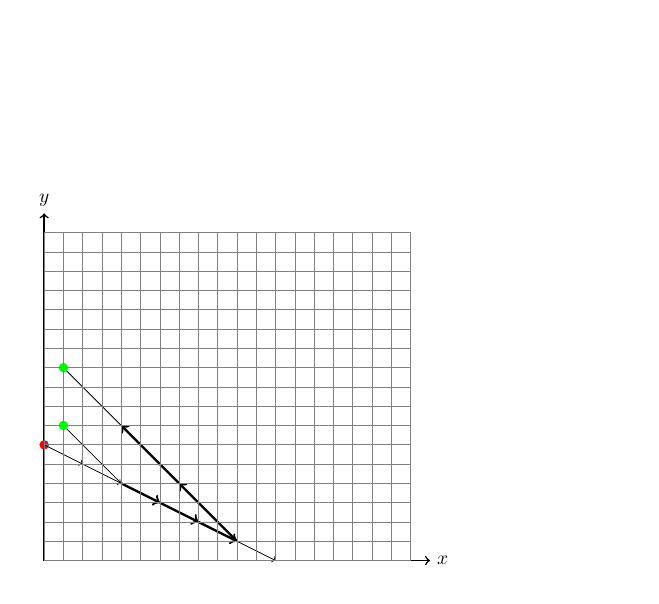
\begin{tikzpicture}[scale=0.35]
\scalebox{0.7}{
\draw[->, thick] (0, 0) -- (20, 0) node[right] {$x$};
\draw[->, thick] (0, 0) -- (0, 18) node[above] {$y$};

\fill[red] (0,6) circle (7pt);

\draw[->] (0,6) -> (2,5);
\draw[->] (2,5) -> (4,4);
\draw[very thick,->] (4,4) -> (6,3);
\draw[very thick,->] (6,3) -> (8,2);
\draw[very thick,->] (8,2) -> (10,1);
\draw[->] (10,1) -> (12,0);

\draw[->] (4,4) -> (1,7);
\fill[green] (1,7) circle (7pt);

\draw[very thick,->] (10,1) -> (7,4);
\draw[very thick,->] (7,4) -> (4,7);
\draw[->] (4,7) -> (1,10);
\fill[green] (1,10) circle (7pt);

\draw[step=1, gray, thin] (0, 0) grid (19, 17);
}
\end{tikzpicture}
\end{minipage}
\begin{minipage}{0.5\textwidth}
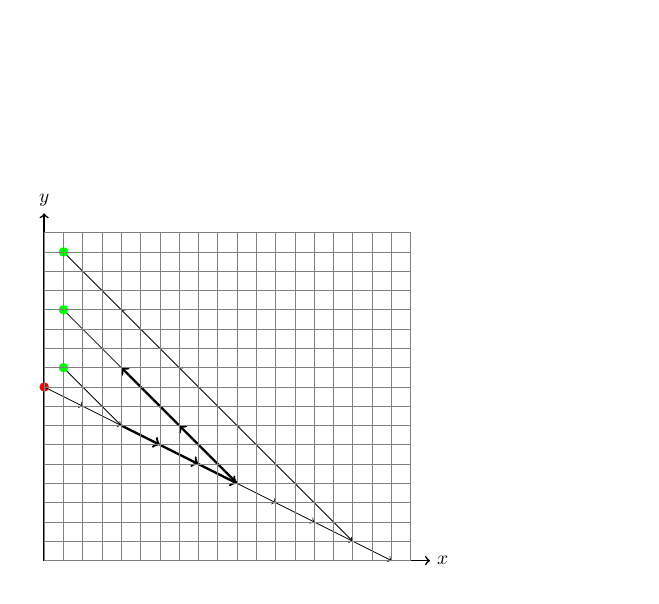
\begin{tikzpicture}[scale=0.35]
\scalebox{0.7}{
\draw[->, thick] (0, 0) -- (20, 0) node[right] {$x$};
\draw[->, thick] (0, 0) -- (0, 18) node[above] {$y$};

\fill[red] (0,9) circle (7pt);

\draw[->] (0,9) -> (2,8);
\draw[->] (2,8) -> (4,7);
\draw[very thick,->] (4,7) -> (6,6);
\draw[very thick,->] (6,6) -> (8,5);
\draw[very thick,->] (8,5) -> (10,4);
\draw[->] (10,4) -> (12,3);
\draw[->] (12,3) -> (14,2);
\draw[->] (14,2) -> (16,1);
\draw[->] (16,1) -> (18,0);

\draw[->] (4,7) -> (1,10);
\fill[green] (1,10) circle (7pt);

\draw[very thick,->] (10,4) -> (7,7);
\draw[very thick,->] (7,7) -> (4,10);
\draw[->] (4,10) -> (1,13);
\fill[green] (1,13) circle (7pt);

\draw[->] (16,1) -> (13,4);
\draw[->] (13,4) -> (10,7);
\draw[->] (10,7) -> (7,10);
\draw[->] (7,10) -> (4,13);
\draw[->] (4,13) -> (1,16);
\fill[green] (1,16) circle (7pt);

\draw[step=1, gray, thin] (0, 0) grid (19, 17);
}
\end{tikzpicture}
\end{minipage}

\caption{Left: $u_2 = 6$, $S_2 = \set{7,10}$. Right: $u_2 = 9$, $S_2 = \set{10,13,16}$.
Thick vectors add up to $p$.}
\label{fig:infix}
\end{figure}

Let $\alpha_1$ and $\alpha_2$ be empty sequences, $\eff(\beta_1) = (2, -1)$ and $\eff(\beta_2) = (-3, 3)$.
Let $u_1 = 0$, $v_1 = 1$. 
The set of solutions $(n_1, n_2)$ of~\eqref{eq:xy} is of the form $w+p^*$, where
$w = (2,1)$ and $p = (3,2)$, and
$\eff_2(p) = 3 \cdot (-1) + 2 \cdot 3 = 3$.
Figure~\ref{fig:infix} shows $R(u_2) = \set{7,10}$ when $u_2 = 6$, and $R(u_2)  = \set{10,13,16}$ when $u_2 = 9$.
In the latter case, elements of $R(u_2)$ correspond to the solutions $w$, $w+p$ and $w+2p$ of~\eqref{eq:xy},
i.e., to $w + kp$ for $k$ in an interval $[0,2]$.
According to Claim~\ref{cl:interval}, this is true in general.
%$S_2 = \setof{u + kp}{k\in I}$, for some interval $I$.
\end{example}

%The following claim states that the number of possible periods $p$ used in the run is an interval.

\begin{claim}\label{cl:interval}
For each $c \in S_1$ there exists an interval $I_{c} = [k_1, k_2]$, where $k_1\in \N$ and $k_2 \in \N_{\infty}$,
such that
$R(c) = \setof{\eff_2(w) + k \cdot \eff_2(p)}{k\in I_{c}}$.
% and path $\rho(b+kp)$ starting from $(b_1, c)$ is a valid if and only if $k \in I_c$. 
\end{claim}

\begin{proof}
It is sufficient to show that whenever $(u_1, c) \trans{w + k_1 \cdot p}$ and
$(u_1, c) \trans{w + k_2 \cdot p}$ for some
$k_1 < k_2 \in \N$,
then
$(u_1, c) \trans{w + k \cdot p}$ for all $k \in [k_1, k_2]$.
Fix $k \in [k_1, k_2]$.
Every point $x$ on the (possibly $\Z$-)path $(u_1, c) \trans{w + k \cdot p}$ is actually on a straight line between some two points,
one on the path $(u_1, c) \trans{w + k_1 \cdot p}$, and the other on the path $(u_1, c) \trans{w + k_2 \cdot p}$.
In consequence $x$, being a weighted average of the two points in $\N^2$, necessarily belongs to $\N^2$. 
Therefore $(u_1, c) \trans{w + k \cdot p}$ is a path.
\end{proof}

We notice that $\eff_2(p)$ can be negative, but this is irrelevant for our arguments.
%
By Claim~\ref{cl:interval}, for each $c \in S_1$ the set $R(c)$ is
is an arithmetic sequence of difference $\essdvass r := \absv{\eff_2(p)}$ and length equal to the cardinality
of the interval $I_{c}$.
%Thus $R(c) = b + (\essdvass r)^{\card{I_c}}$, for some $b\in\N$. 
Let $\spn(c)\in\N_\infty$ be the difference between the supremum of $R(c)$ and the minimal element in $R(c)$.
We say that $\spn(c) = \infty$ if $R(c)$ is infinite.
We split the proof into cases, depending on
whether $\essdvass r$ divides the difference $r$ of the sequence $S_1$, or not.
Additionally we have a case when $\essdvass r = 0$, in other cases we silently assume that $\essdvass r \neq 0$.


\para{Case I: $r$ is divisible by $\essdvass r$}

Therefore, if $\spn(c) \geq r$ then the sequence $R(c)$ actually touches the sequence $R(c+r)$,
i.e., their union is a larger arithmetic sequence of difference $\essdvass r$:

\begin{claim}\label{cl:merged}
If $R(c+r^*) \neq \emptyset$ and $c \geq D:= 3(M+r) \cdot M^2 + M \cdot \norm(w)$,
then $R(c+r^{\leq T}) = b+(\essdvass r)^{\leq T'}$ for some $b \leq c + \eff_2(w) + M \cdot \eff_2(p)$ and $T' \in \N_\infty$.
\end{claim}

\begin{proof}
We first show that $\spn(c) \geq r$.
Suppose $R(c+r^*) \neq \emptyset$ and $c \geq D$.
Due to the first assumption,  for some $n\in\N$ there is a path $(u_1, c+nr) \trans{(n_1, n_2)}$
of the form
\begin{align} \label{eq:Mp}
(u_1, c+nr) \trans{\alpha_1} (\essdvass{x}_1, \essdvass{y}_1) \trans{\beta_1^{n_1}} (\essdvass{x}_2, \essdvass{y}_2) \trans{\alpha_2} (\essdvass{x}_3, \essdvass{y}_3) \trans{\beta_2^{n_2}} (v_1, v_2).
\end{align}
In particular,  $u_1 \geq \drop_1(\alpha_1)$
and therefore $\essdvass x_1\geq 0$.
It is enough to take $(n_1, n_2) := w + Mp$ in \eqref{eq:Mp}.
Then $n_1 \geq M$, so $\essdvass x_2 \geq \essdvass x_1 + M \geq M \geq \drop_1(\alpha_2)$.
Therefore $\essdvass x_3\geq 0$.
Now we show that $c$ is large enough such that $(u_1, c) \trans{w+Mp}$ is nonnegative on the second coordinate as well.
As $\norm(p) \leq 2M$ then $n_1 + n_2 \leq M \cdot \norm(p) + \norm(w) \leq 2M^2 + \norm(w)$. Therefore
$\beta_1^{n_1}$ and $\beta_2^{n_2}$ can in total decrease the second coordinate by at most $M \cdot (2M^2 + \norm(w))$.
As $\alpha_1 + \alpha_2$ can in total decrease the second coordinate by at most $M$ and
$D \geq M + M \cdot (2M^2 + \norm(w))$ we conclude that indeed the path $(u_1, c) \trans{w+Mp}$ is valid.
For the same reasons, for every $m\in [M, M+r]$ there is a path $(u_1, c) \trans{w+mp}$, which guarantees $\spn(c) \geq r$. 

Now we use that fact that $\spn(c) \geq r$.
By monotonicity of \vass, if $R(c) = b+(\essdvass r)^{\leq {T'}}$
then $R(c+r)$ necessarily includes $R(c) + r= b+r+(\essdvass r)^{\leq {T'}}$.
Since $\spn(c) \geq r$, we have $b+r \in R(c)$, but also $b+r \in R(c+r)$,
and therefore the union $R(c) \cup R(c + r)$ forms one arithmetic sequence 
$b+(\essdvass r)^{\leq T'}$, for some $b\in\N$ and $T'$.
The similar reasoning applies to any finite union, namely to $R(c+r^{\leq m})$ for $m\in\N$.
In consequence, for every $T\in \N_\infty$ we have $R(c+r^{\leq T}) = b + (\essdvass r)^{\leq T'}$,
for some $b\in\N$ and $T'\in \N_\infty$,
and since $c+ \eff_2(w) + M \cdot \eff_2(p) \in R(c)$ we get the inequality $b \leq c + \eff_2(w) + M \cdot \eff_2(p)$, as required.
\end{proof}

We are ready for concluding Case I.
%Let $D = 3(M+r) \cdot M^2 + M \cdot \norm(w)$, as in the Claim~\ref{cl:bigspan}.
As $\norm(w) \leq \poly(B, M)$ we have $D \leq \poly(B, M, r)$.
We  partition $S_1 = a + r^{\leq T}$ into two subsets: $S'_1 = S_1 \cap [0,D)$
and $S''_1 = S_1 \cap [D,\infty)$, both being arithmetic sequences of difference $r$,
and consider $S'_1$ and $S''_1$ separately.
 
Concerning $S'_2:= R(S'_1)$,
as $\max(S'_1) \leq D$, all
elements of $S'_2$ are upper-bounded by a polynomial in $M$ and $r$, namely
$\max(S'_2) \leq M^2 \cdot (2M + D)$. 
Thus $S'_2$ can be seen as a finite sum of singletons, each of which
being an $(a', r', T')$-arithmetic sequence with $a' \leq M^2 \cdot (2M + D) \leq \poly(B,M,r)$,
$r' = 1$ and $T' = 0$. 
Clearly $r' = 1 \leq \poly(M)$, and hence $S'_2$ is of the required form.

Now we consider $S''_2:= R(S''_1)$.
If $S''_2 = \emptyset$ we are done.
Otherwise, let $c:= \min(S''_1)$.
Thus $S''_1 = c+r^{\leq T}$ for some $T \in \N_\infty$, 
and $D\leq c \leq \max(a, D+r)$.
%By Claim~\ref{cl:bigspan}, $\spn(c) \geq r$, and therefore using Claim~\ref{cl:neighbours} 
By Claim~\ref{cl:merged} we deduce that
$S''_2 = b + (\essdvass r)^{\leq T'}$ for some 
$b \leq c + \eff_2(w) + M \cdot \eff_2(p)$ and $T' \in \N_\infty'$. 
As $\eff_2(w) \leq \poly(B,M)$, $\eff_2(p) \leq \poly(M)$ and $c \leq a + \poly(B,M, r)$ we get $b \leq a + \poly(B, M, r)$.
We also have $\essdvass r \leq \poly(M)$, and hence
$S''_2$ is of the required form.


\para{Case II: $r$ is not divisible by $\essdvass r$}
%Assume now that $r$ does not divide $\eff_2(p)$. 

In that case we split $S_1 = a + r^{\leq T}$ into several
arithmetic sequences of difference $r \cdot \essdvass r$, namely into sequences of a form 
$(a + m \cdot r) + (r \cdot \essdvass r)^{\leq T'}$, where $m < \essdvass r$, 
and apply the above reasoning to each of this sequences separately. 
As $\essdvass r \leq \poly(M)$
we get also a finite set of arithmetic sequences with the base bounded by $a + \poly(B, M,r)$ and difference bounded by $\poly(M)$,
as required.

\para{Case III: $\essdvass r = 0$}
\Wlog we assume $R(S_1) \neq \emptyset$. For every $c \in S_1$ we have that either $R(c) = c + \eff_2(w)$ or $R(c) = \emptyset$. By monotonicity of VASS we have that if $R(c) \neq \emptyset$ then $R(c+r) \neq \emptyset$. Let $D := 3(M+r) \cdot M^2 + M \cdot \norm(w)$. Similarly as in the proof of Claim~\ref{cl:merged} we observe that if $c \geq D$ then for some $k \in N$ there is a run $(u_1, c) \trans{w+kp}$. Hence we have $R(S_1) = c + \eff_2(w) + r^{\leq T'}$ for some $T' \in \N_\infty$ and some $c \in S_1$ such that $c \leq \max(a, D+r)$. Therefore $R(S_1) = b + r^{\leq T'}$ for some $b \leq a + \poly(B,M,r)$ as required.

\end{proof}



%
%Observe, that if $(b_1, s) \trans \rho (b_2, t)$ for $s \in S_1$ and $t \in S_2$ then $x,y$ satisfy the following equation:
%$$\eff_1(\alpha_1\alpha_2) + x\eff_1(\beta_1) + y\eff_1(\beta_2) = b_2-b_1$$
%Hence we have that the set $S$ of such  pairs $(x,y)$ associated is included in set of solutions of the above equation, which can be represented by Lemma~\ref{lem:taming} as $L(B,P)$ for some sets $B, P \subseteq \N^2$ such that $\norm(B) \leq c(M+B)$ and $\norm(P) \leq cM$ for some constant $c \in \N_+$. We show, that $P$ has only one element $p$. This is because the set of solutions of the following equations over $\Q$ is one dimensional vector space and there is nonnegative solution, because of different signs of $\eff_1(\beta_1)$ and $\eff_1(\beta_2)$:
%$$x\eff_1(\beta_1) + y\eff_1(\beta_2) = 0$$
%Hence each path can be represented as $b+kp$ for some $k \in \N$ and $b \in B$ (recall that with each path we associated pair $(x,y)$). Because $B$ is finite and we are interested in a finite union representation it is enough to show that there exists polynomial $R(M)$ such that the set $S_2' =   \{y_2 \mid \exists_{y_1 \in S_1} (b_1, y_1) \trans{b+kp} (b_2, y_2), k \in \N \}$ is a finite union of $(a', r', T')$-arithmetic sets with $a' \leq a + (B+r) \cdot R(M)$ and
%$r' \leq R(M)$.
%
%We have $p=(p_1, p_2)$ and we write $\eff(p)$ for $\eff(\beta_1^{p_1}\beta_2^{p_2})$. Moreover $b = (b_1, b_2)$ and we write $\eff(b+kp)$ for $\eff(\alpha_1\beta_1^{b_1}\alpha_2\beta_2^{b_2}) + k \eff(p)$. First we solve a case when $|\eff_2(p)|$ divides $r$, to which we will reduce the other case. Let $m = \frac{r}{|\eff_2(p)|}$. Moreover, \mywlog we can assume that $S_2' \neq \emptyset$.
%The intuition is that the set $S_2'$ will be a condensing of $S_1$ due to repetitions of $p$ with base point $a'$ moved a bit. In order to conclude the prove we need a few claims. 
%\begin{claim}
%For each $s \in S_1$ there exists interval $I = [k_1, k_2]$ such that $k_1, k_2 \in \N_{\infty}$ and path $b+kp$ starting from $s$ is a valid path if and only if $k \in I$. 
%\end{claim}
%\begin{proof}
%It is enough to show, that if for $k_1 < k_2 \in \N$ we know, that $b+k_1p$ and $b+k_2p$ are valid paths starting from $s$ then for all $k_3 \in [k_1, k_2]$ we have that path $b+k_3p$ is a valid path starting from $s$. Let us fix $k_3 \in [k_1, k_2]$ and let $b=(b_1, b_2), p=(p_1, p_2) \in \N^2$. Recall, that $\eff(\beta_1) \in \N_+ \times \N_-$ and $\eff(\beta_2) \in \N_- \times \N_+$. Hence it is enough to show the following inequalities:
%$$\eff_1(\alpha_1\beta_1^{b_1+k_3p_1}\alpha_2\beta_2^{b_2+k_3p_2}) = \eff_1(\alpha_1\beta_1^{b_1+k_1p_1}\alpha_2\beta_2^{b_2+k_1p_2})$$
%$$\eff_2(\alpha_1\beta_1^{b_1+k_3p_1}) \geq \eff_2(\alpha_1\beta_1^{b_1+k_2p_1})$$
%For the first equality observe, that:
%\begin{align*}
%\eff_1(\alpha_1\beta_1^{b_1+k_3p_1}\alpha_2\beta_2^{b_2+k_3p_2}) & = \eff_1(\alpha_1\beta_1^{b_1+k_1p_1}\alpha_2\beta_2^{b_2+k_1p_2}) 
%+ (k_3-k_1)(p_1\eff_1(\beta_1) + p_2\eff_1(\beta_2)) \\
%& = \eff_1(\alpha_1\beta_1^{b_1+k_1p_1}\alpha_2\beta_2^{b_2+k_1p_2})
%\end{align*}
%The second inequality follows from the fact that:
%$$b_1+k_3p_1 \leq b_1+k_2p_1$$
%\end{proof}
%Let us by $I_x = [k_1^s, k_2^s]$ denote the interval for $x \in S_1$ and by $|I_x| = k_2^s - k_1^s$. Now we split elements of $S_1$ into three groups depending on the properties of the points in $S_1$.
%\begin{claim}\label{clm:split}
%For each $x \in S_1$ at least one of the following holds:
%\begin{itemize}
%\item $x \leq a + 3cM^2(B+r)$
%\item $x$ is the maximal element of $S_1$ and $[0,m] \subseteq I_x$
%\item $[0, m] \subseteq I_x$ and if $b+kp$ is executable from $(b_1,x)$ for $k > m$ than $b+(k-m)p$ is executable from $(b_1,x+m\eff_2(p))$ and $x+m\eff_2(p) \in S_1$. 
%\end{itemize}
%\end{claim}
%\begin{proof}
%Let us take $x \in S_1$ such that  $x > a + 3cM^2(B+r)$. Firstly, we show that $[0, m] \subseteq I_x$. Recall, that $\Lambda$ is one-turn and observe, that for all $k \in \N$ we have:
%$$\eff_1(\alpha_1\beta_1^{b_1}\alpha_2\beta_2^{b_2}) = \eff_1(\alpha_1\beta_1^{b_1}\alpha_2\beta_2^{b_2}) + k(p_1\eff_1(\beta_1) + p_2\eff_1(\beta_2))$$
%Hence, because $S_2$ is not empty we have that all paths $b+kp$ starting from $(b_1, x)$ are valid on the first counter. Hence we only need to deal with the second counter. Now observe, that for each $k \in [0,m]$ we have that maximal decrease of the second counter along path $b+kp$ is at most :
%\begin{align*}
%M + (b_1+kp_1)\eff_2(\beta_1) & \leq M + (c(M+B)+mcM)M \\
%& \leq 3cM^2(B+m) \leq 3CM^2(B+r) < x
%\end{align*}
%Hence $[0, m] \subseteq I_x$.
%If $x$ is the maximal element we are done. Otherwise,
%we show, that if $b+kp$ is executable from $(b_1,x)$ for $k > m$ than $b+(k-m)p$ is executable from $(b_1,x+m\eff_2(p))$ and $x+m\eff_2(p) \in S_1$. Observe, that $x+m\eff_2(p) = x+r$ if $\eff_2(p) > 0$ and $x+m\eff_2(p) = x-r$ otherwise. Because $S_1 =  a + r^{\leq K}$ and $x$ is not the maximal element of $S_1$ then in the first case $x+m\eff_2(p) \in S_1$. In the second case we have $x -  r \geq a+r-r \geq a$ and hence $x-r \in S_1$.
%
%Now it is left, that $b+(k-m)p$ is executable from $(b_1,x+m\eff_2(p))$. Similarly as before we only need to take care about the second counter. For this it is enough to observe, that:
%\begin{align*}
%x + m\eff_2(p) + \eff_2(\alpha_1\beta_1^{b_1+(k-m)p_1}) 
%& = x + \eff_2(\alpha_1\beta_1^{b_1+kp_1}) + mp_2\eff_2(\beta_2) \\
%& \geq x + \eff_2(\alpha_1\beta_1^{b_1+kp_1})
%\end{align*}
%This is due to $\eff_2(p) = p_1\eff_2(\beta_1) + p_2\eff_2(\beta_2)$ and $\eff_2(\beta_2) \geq 0$.
%Moreover:
%$$x+m\eff_2(p) \geq a+3cM^2(B+r)-r \geq a + M \geq |\eff_2(\alpha_1)|$$
%\end{proof}
%Now we can split $S_1$ into three parts $A_1, A_2, A_3$ such that elements from $A_1$ are the one with $s \leq a + 3cM^2(B+r)$, $A_3$ is the singleton or empty set containing the maximal element and $A_2$ is the rest of $S_1$. Observe, that $A_2 = a_2+r^{\leq K}$ for $a_2 \leq 3cM^2(B+r) + r, a_2 = a + kr$ for some $k \in \N$ and $K = T - k - 1$. Moreover observe, that if path start from $s \in A_2$ and is of the form $b+kp$ for $k > m$ than the same point is reachable from point $(b_1,s+m\eff_2(p))$ by path $b+(k-m)p$ due to Claim \ref{clm:split}. Hence, because we can iterate the argument at some point the starting point will be in $A_1 \cup A_3$ or $k \leq m$. Hence for points from $A_2$ we only need to consider paths $b+kp$ for $k \leq m$. Let us define $B_1, B_2$ and $B_3$.  
%$$B_1 = \bigcup_{x \in A_1, k \in I_x} \set{x + \eff_2(b+kp)}$$
%$$B_2 = \bigcup_{x \in A_2, k \in [0,m]} \set{x + \eff_2(b+kp)} 
%= a_2 + r^{\leq T} + \eff_2(b) + \eff_2(p)^{\leq m}$$
%$$B_3 = \bigcup_{x \in A_3, k \in I_s} \set{x + \eff_2(b+kp)}$$ 
%Which if $A_3 \neq \emptyset$ can be represented as
%$$B_3= a + (T+1)r  + \eff_2(b) + \eff_2(p)^{\leq |I_{x_{max}}|}$$
%where $x_{max}$ is the element of $A_3$. From now on we fix this maximal element and put $|I_{x_max}| = 0$ if it does not exist. 
%Let us observe:
%$$S_2 = B_1 \cup B_2 \cup B_3$$
%We deal separately with $B_1$ and $B_2 \cup B_3$. Because $a_2 + \eff_2(b) \leq 3cM^2(B+r) + r $ clearly, in order to show, that $B_2 \cup B_3$ is  of the form we want it is enough to show the following claim (recall that $\eff_2(p)$ can not be zero due to divisibility condition):
%\begin{claim}
%$(B_2 \cup B_3) \cap [a_2 + \eff_2(b), \infty] = a_2 + \eff_2(b) + |\eff_2(p)|^{\leq T'}$ where $T' = m(T+1) + |I_{x_{max}}|$ if $\eff_2(p) > 0$ and $T' = m(T+1)$ if $\eff_2(p) < 0$ .  
%\end{claim}
%\begin{proof}
%Firstly we show $(B_2 \cup B_3) \cap [a_2 + \eff_2(b), \infty] \subseteq a_2 + \eff_2(b) + |\eff_2(p)|^{\leq T'}$. Let us take any $x \in (B_2 \cup B_3) \cap [a_2 + \eff_2(b), \infty]$. The first case is that $x \in B_2$ and hence 
%$$x = a_2 + \eff_2(b) + k_1r + k_2\eff_2(p)$$
%for $k_1 \leq T$ and $k_2 \leq m$. We have 
%$$x = a_2 + \eff_2(b) + k_1m|\eff_2(p)| + k_2\eff_2(p)$$
%and hence if $\eff_2(p) > 0$ we have 
%$$x = a_2 + \eff_2(b) + (k_1m + k_2)|\eff_2(p)| \in a_2 + \eff_2(b) + |\eff_2(p)|^{\leq T'}$$
%and if $\eff_2(p) < 0$ we have 
%$$x =  a_2 + \eff_2(b) + |\eff_2(p)|^{k_1m-k_2}$$
%Because $x \geq a_2 + \eff_2(b)$ we have $k_1m-k_2 \geq 0$ and hence $x \in a_2 + \eff_2(b) + |\eff_2(p)|^{\leq T'}$ .
%
%Now we show $a_2 + \eff_2(b) + |\eff_2(p)|^{\leq T'} \subseteq (B_2 \cup B_3) \cap [a_2 + \eff_2(b), \infty]$. Let us take $x = a_2 + \eff_2(b) + k|\eff_2(p)|$ for some $k \leq T'$. Firstly let us consider case when $\eff_2(p) > 0$. 
%\begin{align*}
%x & = a_2 + \eff_2(b) + \floor{\frac{k}{m}}m|\eff_2(p)|+ (k\mod m)|\eff_2(p)| \\
%& = a_2 + \eff_2(b) + \floor{\frac{k}{m}}r + (k \mod m)\eff_2(p)
%\end{align*}
%Observe, that if $k \leq m(T+1)$ we have
%$$\floor{\frac{k}{m}} \leq \floor{\frac{m(T+1)}{m}} = T+1$$
%Hence $x \in a_2 + \eff_2(b) + r^{\leq T} + |\eff_2(p)|^{\leq m} = B_2$
%If $k > m(T+1)$ then observe, that $k - m(T+1) \leq |I_{x_{max}}|$ and see, that
%$$x = a_2 + \eff_2(b) + r(T+1) + \eff_2(p)^{k-m(T+1)} \in B_3 $$
%
%Now we consider case when $\eff_2(p) < 0$. Then:
%$$x=a_2 + \eff_2(b) + \ceil{\frac{k}{m}}m|\eff_2(p)|-(m - (k \mod m))|\eff_2(p)|$$
%Then if $k \leq mT$ we have:
%$$x \in a_2 + \eff_2(b) + r^{\leq T}+\eff_2(p)^{\leq m} = B_2 $$
%And if $k > mT$ we have:
%$$x \in a_2 + \eff_2(b) + (T+1)r + \eff_2(p)^{\leq m} \subseteq B_3$$
%
%\end{proof}
%For the set $B_1$ it is enough to prove the following Claim:
%\begin{claim}
%$B_1$ can be represented as a finite union of $(a', r',T')$-arithmetic sets with $a' \leq a + 10cM^4(B+r)$ and $r' \leq cM$.
%\end{claim}
%\begin{proof}
%The first case is that the second counter is at most $3cM^2(B+r)$ at the beginning. The first counter is at most $B$ at the beginning. Then after $\alpha_1$ they are at most $3cM^2(B+r) + M \leq 4cM^2(B+r)$. Then after all execution of the $\beta_1$ the sum of the counters is at most $8cM^3(B+r)$ then after $\alpha_2$ the sum of counters is at most $8cM^3(B+r) + 2M$ and finally after the last execution of $\beta_2$ the sum of counters and hence also the second counter is at most $8cM^4(B+r) + 2M^2 \leq 10cM^4(B+r)$ as needed. Hence there is a finite number of such elements and they can be represented as a singleton arithmetic sets.
%The second case is that the second counter is at least $3cM^2(B+r)$ at the beginning. Let the beginning point be $x$. We show, that elements of $B_1$ obtained by the paths starting in $x$ can be represented as an arithmetic-set. Therefore assume this set is not empty (otherwise it is trivial). Recall, that $\Lambda$ is one-turn and observe, that for all $k \in \N$ we have:
%$$\eff_1(\alpha_1\beta_1^{b_1}\alpha_2\beta_2^{b_2}) = \eff_1(\alpha_1\beta_1^{b_1}\alpha_2\beta_2^{b_2}) + k(p_1\eff_1(\beta_1) + p_2\eff_1(\beta_2))$$
%All paths $b+kp$ starting from $x$ are valid on the first counter. Hence we only need to deal with the second counter. Now observe, that  we have that maximal decrease of the second counter along path $b$ is at most :
%$$M + b_1\eff_2(\beta_1) \leq M + c(M+B)M \leq 3cM^2B$$ Hence path $b$ is also valid on the second counter. Hence $x_2 + \eff_2(b) \in B_1$ and $x_2 + \eff_2(b) \leq a + 3cM^2(B+r) + \eff_2(\alpha_1\alpha_2) + b_1\eff_2(\beta_1) + b_2\eff_2(\beta_2) \leq a + 3cM^2(B+r) + M +  2c(M+B)M \leq a + 10cM^2(B+r)$. Now if $\eff_2(p) > 0$ then the set can be represented as $(x_2 + \eff_2(b), \eff_2(p), T')$-arithmetic set, which satisfies the conditions. Otherwise all elements are at most $a + 10cM^2(B+r)$ and can be represented as singleton arithmetic sets, which satisfies the conditions.
%\end{proof}
%By previous claims we know, that $S_2$ is a finite union of $(a',r', T')$-arithmetic sets for $a' \leq a + 10cM^4(B+r)$ and $r' \leq cM$.
%
%
%Now we come back to the case when $r$ is not divisible by $|\eff_2(p)|$. The first subcase is that $\eff_2(p) = 0$. Then all paths $b+kp$ have the same effect so we only need to consider path $b$. The lowest $x \in S_1$ from which the path $b$ is executable is at most $M + b_1\eff_2(\beta_1) + a + r \leq M + c(M+B)M + a+r \leq a + 3M^2(B+r)$. Hence set $S_2$ can be represented as $(a', r, T')$-arithmetic set for $a' \leq a+ 3M^2(B+r) + \eff_2(b) \leq a+ 3M^2(B+r) + M+2c(M+B)M \leq a + 10M^2(B+r)$. The second subcase is that $\eff_2(p) \neq 0$. Then we can split $S_1$ into several $(a'', \eff_2(p)r, T'')$-arithmetic sets with $a'' \leq a + \eff_2(p)r \leq a + (2cM^2+M)r$ then we can apply the first case and get representation of $S_2$ as a finite union of $(a',r', T')$-arithmetic sets with $r' \leq cM$ and $a' \leq a + (2cM^2+M)r + 10cM^4(B+r) \leq a+ 13M^4(B+r)$. Thus by setting $R(M) = 13cM^4$ we conclude the proof. 
%\end{proof}

This work identifies signal collapse as a critical bottleneck in one-shot neural network pruning. Performance loss in pruned networks is due to \textbf{signal collapse} in addition to the removal of critical parameters. We propose \textbf{REFLOW} (\textbf{Re}storing \textbf{F}low of \textbf{Low}-variance signals), a simple yet effective method that mitigates signal collapse without computationally expensive weight updates. By focusing on signal preservation, REFLOW highlights the importance of mitigating signal collapse in sparse networks and enables magnitude pruning to match or surpass state-of-the-art one-shot pruning methods such as CHITA, CBS, and WF.

REFLOW consistently achieves state-of-the-art accuracy across diverse architectures, restoring ResNeXt-101 from under 4.1\% to 78.9\% top-1 accuracy at 80\% sparsity on ImageNet. Its lightweight design makes it a practical solution for both research and deployment, delivering high-quality sparse models without the overhead of traditional approaches. These findings challenge the traditional emphasis on weight selection strategies and underscore the critical role of signal propagation for achieving high-quality sparse networks in the context of one-shot pruning.





\subsection{Plasticity in Neural Networks}
In recent years, various methods have been proposed to address plasticity loss.
Several works have focused on maintaining active units \cite{abbas2023loss, elsayed2024addressing} or re-initializing dead units \cite{sokar2023dormant, dohare2024loss}.
Other studies have explored limiting deviations from the initial statistics of model parameters \cite{kumar2023maintaining, lewandowski2023curvature, elsayed2024weight}.
Additionally, some methods rely on architectural modifications \cite{nikishin2024deep, lee2024slow, lewandowski2024plastic}.  
Plasticity loss also occurs in the reinforcement learning due to its inherent non-stationary. \citet{nikishin2022primacy} proposed resetting the model, while \citet{asadi2024resetting} suggested resetting the optimizer state. 

As noted by \citet{berariu2021study}, loss of plasticity can be divided into two distinct aspects: a decreased ability of networks to minimize training loss on new data (trainability) and a decreased ability to generalize to unseen data (generalizability).
While most previous works focused on trainability, \citet{lee2024slow} addressed generalizability loss.
They demonstrated that plasticity loss also occurs under a stationary distribution, as in a warm-start learning scenario where the model is pretrained on a subset of the training data and then fine-tuned on the full dataset.

Most existing studies have focused on only one of the following challenges: trainability, generalizability, or reinforcement learning.
However, in this study, we validate our AID method across all three aspects, demonstrating its effectiveness in each scenario.



\subsection{Activation Function}
Our AID method is a stochastic approach similar to Dropout while also functioning as an activation function.
Therefore, we aim to discuss previously proposed probabilistic activation functions.
Although the field of probabilistic activation functions has not seen extensive research, two noteworthy studies exist.
The first is the Randomized ReLU (RReLU) function, introduced in the Kaggle NDSB Competition \cite{xu2015empirical}.
The original ReLU function maps all negative values to zero, whereas RReLU maps negative values linearly based on a random slope.
During testing, negative values are mapped using the mean of the slope distribution.
Their experimental results suggest that RReLU effectively prevents overfitting.
Another example of a probabilistic activation function is DropReLU \cite{liang2021drop}.
DropReLU randomly determines whether a node's activation is processed through a ReLU function or a linear function.
The authors claim that DropReLU improves the generalization performance of neural networks.
The fundamental distinction between these probabilistic activation functions and our method lies in the generality of our approach.
Unlike simple probabilistic activation functions, our method encompasses techniques such as Dropout and ReLU, providing a more comprehensive framework.

Another related approach involves activation functions designed to address plasticity loss.
\citep{abbas2023loss} proposed the Concatenated Rectified Linear Units (CReLU), which concatenates the outputs of the standard ReLU applied to the input and its negation.
This structure prevents the occurrence of dead units, thereby improving plasticity.
Additionally, trainable activation functions have also been shown to effectively mitigate plasticity loss in reinforcement learning \citep{delfosseadaptive}.
Specifically, they introduced a trainable rational activation function that prevents value overfitting and overestimation in reinforcement learning.



\begin{figure*}[ht!]
    \centering
    \includegraphics[width=0.3\textwidth]{figures/sources/mainnet_pls_acc.pdf}
    \includegraphics[width=0.3\textwidth]{figures/sources/subnet_pls_acc.pdf}
    \includegraphics[width=0.3\textwidth]{figures/sources/warm_start_dropout.pdf}
    \caption{\textbf{Left.} Random label MNIST experiment using an 8-layer MLP. Higher dropout probabilities result in significant trainability loss. 
    \textbf{Middle.} Accuracy of the subnetworks trained on random target. Each subnetworks are sampled from original network after each epoch. Subnetworks of the Dropout also experience trainability loss. \textbf{Right.} Warm-start scenario of Resnet-18 model with CIFAR100 dataset. Dropout improves generalization performance; however, the reduction in accuracy compared to the cold-start scenario is nearly identical to that of the vanilla model.}
    \label{exp_dropout}
\end{figure*}




\section{Dataset and Training Details}
\label{app:dataset_n_train}

\subsection{Dataset Generation for Offline Training}
\begin{figure}[t]
    \centering
    \includegraphics[width=\linewidth]{images/entity_label.pdf}
    \vspace{-1.5pc}
    \caption{Illustration of our entity-level dataset construction. We form entity-level hallucination labels according to the atomic facts extracted by \textsc{FActScore}.}
    \label{fig:data_generation}
    \vspace{-1pc}
\end{figure}

The Multiturn-aware Reward (MR) function enables the generation of high-quality synthetic conversation datasets for training. Given a user query, multiple LLM responses are sampled and ranked based on their MR scores, with higher-ranked responses designated as \textit{Chosen} and lower-ranked as \textit{Rejected}. To simulate natural conversational flow, the first turn from the chosen response's forward interaction window is appended to the prompt for the next turn, iteratively extending the conversation until completion. Solid red arrows denote data collection for Supervised Fine-Tuning (SFT), while dashed blue arrows indicate preference data construction for Direct Preference Optimization (DPO). This approach systematically curates multiturn conversations that enhance both response quality and collaborative efficiency, both of which are explicitly captured by MR.

Given (1) a user simulator LLM, \eg GPT-4o-mini, (2) an assistant LLM, GPT-4o, and (3) arbitrary tasks with defined task-specific metric, we can simulated and generate high-quality conversations following Figure~\ref{fig:flow}. We create the following training datasets in this simulated environments. 
\small
\begin{tabular}{p{6.8cm}p{.8cm}p{.8cm}p{.8cm}crr}
\toprule
\multirow{2}{*}{\textbf{Metric}} & \multicolumn{3}{c}{\textbf{Median}} & \multicolumn{3}{c}{\textbf{Statistics}} \\
\cline{2-7}
 & \textbf{Iter. 1} & \textbf{Iter. 2} & \textbf{Iter. 3} & \textbf{Comparison} & \textbf{r} & \textbf{p-value} \\
\midrule
\multirow{3}{*}{UMUX-LITE (SUS)} & \multirow{3}{*}{60.82} & \multirow{3}{*}{66.23} & \multirow{3}{*}{82.48} & 1 vs 2 & 1.429 & 0.279 \\
 &  &  &  & 2 vs 3 & 0.000 & 0.066 \\
 &  &  &  & 1 vs 3 & 0.000 & 0.031* \\
\hline
\multirow{3}{*}{NASA-TLX Score} & \multirow{3}{*}{3.92} & \multirow{3}{*}{2.83} & \multirow{3}{*}{1.92} & 1 vs 2 & 2.041 & 0.500 \\
 &  &  &  & 2 vs 3 & 0.817 & 0.138 \\
 &  &  &  & 1 vs 3 & 0.000 & 0.094 \\
\midrule
\multicolumn{7}{c}{\textbf{Self-Defined Likert Scale Questions}} \\
\midrule
\multirow{3}{*}{\makecell[l]{Iterating on my sketches was easy}} & \multirow{3}{*}{4.0} & \multirow{3}{*}{5.0} & \multirow{3}{*}{6.5} & 1 vs 2 & 3.674 & 0.844 \\
 &  &  &  & 2 vs 3 & 0.000 & 0.039* \\
 &  &  &  & 1 vs 3 & 1.429 & 0.156 \\
\hline
\multirow{3}{*}{\makecell[l]{The sketches encapsulated what I intended to achieve}} & \multirow{3}{*}{5.5} & \multirow{3}{*}{5.5} & \multirow{3}{*}{5.5} & 1 vs 2 & 2.654 & 0.783 \\
 &  &  &  & 2 vs 3 & 0.408 & 0.655 \\
 &  &  &  & 1 vs 3 & 1.414 & 0.688 \\
\hline
\multirow{3}{*}{\makecell[l]{The re-generated code aligned with my intended changes}} & \multirow{3}{*}{4.5} & \multirow{3}{*}{5.0} & \multirow{3}{*}{6.0} & 1 vs 2 & 1.225 & 0.892 \\
 &  &  &  & 2 vs 3 & 0.000 & 0.141 \\
 &  &  &  & 1 vs 3 & 0.707 & 0.063 \\
\hline
\multirow{3}{*}{\makecell[l]{I felt more control over the AI model and generated results}} & \multirow{3}{*}{5.5} & \multirow{3}{*}{5.0} & \multirow{3}{*}{5.5} & 1 vs 2 & 2.236 & 0.786 \\
 &  &  &  & 2 vs 3 & 0.000 & 0.785 \\
 &  &  &  & 1 vs 3 & 0.500 & 1.000 \\
\hline
\multirow{3}{*}{\makecell[l]{I felt more control over the whole code editing process}} & \multirow{3}{*}{5.0} & \multirow{3}{*}{5.0} & \multirow{3}{*}{6.0} & 1 vs 2 & 0.000 & 1.000 \\
 &  &  &  & 2 vs 3 & 0.866 & 0.059 \\
 &  &  &  & 1 vs 3 & 1.000 & 0.102 \\
\bottomrule
\end{tabular}


\subsection{Training Details}

We provide the hyperparameters for \name{} fine-tuning in Table~\ref{tab:hyper}. 

Notably, \name{} relies on a minimal set of hyperparameters, using the same window size and sample size for computing MRs across multiple datasets. The penalty factor on token count, $\lambda$, is set lower for \doc compared to \code and \mathc, as document lengths in \doc can vary significantly and may be easily bounded by 1 in Eq.~\ref{eq:intrinsic} if $\lambda$ is too large.
\begin{table}[h!]
    \caption{Hyperparameters}
    \label{tab:TrainingParams}
    \centering
    \begin{tabular}{l|l}
        \textbf{Parameters} & \textbf{Tuning} \\% & \textbf{Estimation}  \\
        \hline
        Sampling time                   & $0.05$  \\   %& $0.05$     \\
        Reward discount factor $\gamma$ & $0.99$  \\   %& $0.99$     \\
        Learning rate for actor         & $10^{-3}$ \\% & $10^{-3}$  \\
        Learning rate for critic        & $10^{-3}$ \\% & $10^{-3}$  \\
        $L_2$ Regularization factor     & $10^{-5}$ \\% & $10^{-4}$  \\
        Optimizer parameter $\epsilon$  & $10^{-8}$ \\% & $10^{-8}$  \\
        Minimum batch size              & $1024$  \\%   & $64$     \\
        Experience buffer length        & $10^{6}$  \\% & $10^{6}$   \\
    \end{tabular}
\end{table}
\begin{tabular}{l l l l l l}
\toprule
\multirow{2}{*}{Task} & \multirow{2}{*}{Pool} & \multicolumn{4}{c}{Sequence} \\ \cmidrule(lr){3-6}
                      &                       & Prompt & Task & Completed & Combined \\
\midrule
Sorting & Int                     & 5 3 6      & S R A E    & 3 5 6         & Q 5 3 6 S R A E 3 5 6        \\
Adding  & Int                     & 5 3 6      & A E R S    & 6 4 7         & Q 5 3 6 A E R S 6 4 7        \\
Reverse Sorting  & Int                     & 5 3 6      & R E A S    & 6 5 3         & Q 5 3 6 R E A S 6 5 3        \\
Even-Odd  & Int                     & 5 3 6      &  E R A S    & 6 3 5         & Q 5 3 6 E R A S 6 3 5        \\
Sorting & Int + Char                     & 13 5 c a      & S E R A    & 13 5 a c & Q 13 5 c a S E R A        \\
Adding  & Int + Char                     & 13 5 c a      & A S R E    & 14 6 d b         & Q 13 5 c a A S R E        \\
Reverse Sorting  & Int + Char                     & 13 5 c a      & R E A S    & c a 5 13         & Q 13 5 c a R E A S c a 5 13        \\
Even-Odd  & Int + Char                     & 13 5 c a      & E S A R    & a c 13 5 & Q 13 5 c a E S A R 13 5 c a        \\

\bottomrule
\end{tabular}% 

\section{Steering details: prompts, datasets, and parameters}
\label{app: prompts}

We now describe the parameters and prompts used for steering Llama-3.1-8B-it and Gemma-2-9B-it toward different concepts.

\subsection{Our prompting method}

We consider a specific example to explain our prompting method, where we extract directions to induce different identities from the surname `Newton'. To extract semantically meaningful directions from the activation spaces of LLMs for steering, we first choose a list of labeled prompts for a list of desired concepts, similar to the approaches of \citet{representation_engineering, turner2023activation}. However, unlike their methods, our prompts do not need to consist of contrastive pairs of positive and negative examples. Further, we found benefit in some cases by choosing prompts to be from real text, and not synthetic datasets. For example, we extracted meaningful concepts corresponding to political positions and disambiguating word meanings from pairs of Wikipedia articles. 

Consider the specific case of distinguishing Cam Newton versus Isaac Newton (Figure~\ref{fig: rfm/pca newton, llama-3.1-8B}). We obtain sentences from the Isaac and Cam Newton wikipedia articles. 
Suppose we want to learn the vector for `Isaac' Newton. Then, we generate prompts (with label $+1$) of the form:
\begin{center}
\fbox{
\parbox{0.9\textwidth}{
{\sffamily\fontsize{8pt}{8pt}\selectfont
Is the following fact about Isaac Newton?\\
Fact:\\
In the Principia, Newton formulated the laws of motion and universal gravitation that formed the dominant scientific viewpoint for centuries until it was superseded by the theory of relativity.}
}
}
\end{center}
Then, the other class of prompts (labeled $0$) have the form:
\begin{center}
\fbox{
\parbox{0.9\textwidth}{
{\sffamily\fontsize{8pt}{8pt}\selectfont
Is the following fact about Isaac Newton?\\
Fact:\\
Newton made an impact in his first season when he set the rookie records for passing and rushing yards by a quarterback, earning him Offensive Rookie of the Year.}
}
}
\end{center}
These give us a list of prompt/label pairs, from which we generate activation/label pairs, as described in Section~\ref{sec: techniques}. We then solve RFM (or another layer-wise predictor) on each layer to predict the label function (Isaac vs. Cam Newton). For RFM, the concept vectors at each layer $c_\ell$ are then the top eigenvectors of the AGOP from each RFM predictor.

\subsection{Human Languages} For triggering language switches as in Figures~\ref{fig: english_chinese, llama-3.1-8B} and \ref{fig: english_spanish, llama-3.1-8B}, we used examples generated from the following prompt template.

\begin{center}
\fbox{\parbox{0.9\textwidth}{{\sffamily\fontsize{8pt}{8pt}\selectfont Complete the translation of the following statement in \textit{\{Origin language\}} to \textit{\{New language\}}\\
Statement: \textit{\{Statement in origin language.\}}\\ Translation: \textit{\{Partial translation in new language.\}} }
}
}
\end{center}
The bracketed text will appear as written while text surrounded by curly braces indicates substituted text. We obtained list of statements in the origin and new languages from datasets of translated statements. To generate the partial translations we truncated translations to the first half of the tokens. For Spanish/English translations we used datasets from \url{https://github.com/jatinmandav/Neural-Machine-Translation/tree/master}. For Mandarin/English, we obtained pairs of statements from \url{https://huggingface.co/datasets/swaption2009/20k-en-zh-translation-pinyin-hsk}. 

To evaluate translations for human language, we use OpenAI's o1 reasoning model to generate a list of 100 English statements and questions. We then evaluate the translation from steering of each sentence.

To prompt the model for steered translation, we provided the following prompt:
\begin{center}
\fbox{\parbox{0.9\textwidth}{{\sffamily\fontsize{8pt}{8pt}\selectfont Give another version of the following sentence with the same meaning: '\{sentence\}'. Write the version in quotes.}
}
}
\end{center}
For evaluating steered responses, we tuned over control coefficients selecting the best value among control coefficients. We steer the outputs of all blocks of the transformer. For Llama-3.1-8B-it, we tuned over coefficients: 0.2, 0.3, 0.4, 0.5, 0.6, 0.7, and for Gemma-2-9B-it: 4.0, 5.0, 6.0, 7.0, 8.0, 9.0. Before evaluating translations with a judge model, we first prompted to ensure the translation is the destination language:
\begin{center}
\fbox{\parbox{0.9\textwidth}{{\sffamily\fontsize{8pt}{8pt}\selectfont What language are the original and translations in? Give your answer in the format '\{Original language\}, \{Translation language\}'. If the translation is empty, assume Language 2 is English."}
}
}
\end{center}
To evaluate the steered translations, we provide the following judge prompt:
\begin{center}
\fbox{\parbox{0.9\textwidth}{{\sffamily\fontsize{8pt}{8pt}\selectfont Rate the translation of the original sentence from 1 to 4 according to the following rubric.\\\\
Score of 1: The translation is mostly inaccurate or unrelated.\\
Score of 2: The translation is slightly unrelated to the original.\\
Score of 3: The translation has mostly the same meaning as the original.\\
Score of 4: The translation has the same meaning as the original.\\\\
Give your response in the format '{score}/4.' Do not penalize awkward or excessive wording. If the translation is empty, give a score of 0.\\
----------------------------------------\\
ORIGINAL: \{original\}\\
----------------------------------------\\
TRANSLATION: \{translation\}"}
}
}
\end{center}

\subsection{Poetry} Prompts for poetry followed the same format as human languages. We obtained 100 pairs of standard English sentences and poetic translations from OpenAI's o1 model. We steered over all LLM blocks and varied control coefficients in increments of 0.1 over 0.4 to 0.8. Figure~\ref{fig: steered poetry style} uses coefficient 0.6. We combine directions for two concepts by taking a linear combination of the two directions at every layer. For poetry and dishonesty (Figure~\ref{fig: main figure}), we use $a=1.2,b=1.0$ as the multiple for each concept, respectively, then use coefficient $0.4$ on the combined vector across all blocks. 

\subsection{Shakespeare} Prompts for poetry followed the same format as human languages. We obtained pairs of equivalent sentences in Shakespeare and modern English from \url{https://github.com/harsh19/Shakespearizing-Modern-English/tree/master}. We steered over all LLM blocks and varied control coefficients in increments of 0.1 over 0.4 to 0.8. For Shakespeare and harmful (Figure~\ref{fig: main figure}), we use $a=1.0,b=0.5$ as the multiple for each concept, respectively, then use coefficient $0.5$ on the combined vector across all blocks. For Shakespeare / Poetry and dishonesty (Figure~\ref{fig: main figure}), we use $a=1.2,b=1.0$ as the multiple for each concept, respectively, then use coefficient $0.4$ on the combined vector across all blocks.

\subsection{Programming Languages}

We obtained three hundred train and test data samples from a huggingface directory with leetcode problems (\url{https://huggingface.co/datasets/greengerong/leetcode}). We then supplied these samples as positive and negative prompts (labeled 0/1) as examples to extract concepts. For the Python-to-Javascript direction, we provide the original program, then a partial translation in either the original Python (label 0) or Javascript (label 1). The partial translation was truncated to half the original length. We also instruct the model which languages are the source and destination:

\begin{center}
\fbox{
   \parbox{0.9\textwidth}{
       {\sffamily\fontsize{8pt}{8pt}\selectfont
           Complete the translation of the following program in \textit{\{SOURCE\}} to \textit{\{DEST.\}}.\\
           Program:\\
           \textit{\{Code in origin language.\}}\\
           Translation:\\
           \textit{\{Partially translated code in dest. language.\}}
       }
   }
}
\end{center}


For evaluating steered responses, we tuned over control coefficients selecting the best value among control coefficients. We steer the outputs of all blocks of the transformer. For Llama-3.1-8B-it, we tuned over coefficients: 0.4, 0.5, 0.6, 0.7, 0.8, and for Gemma-2-9B-it: 4.0, 5.0, 6.0, 7.0, 8.0, 9.0. To prompt the model for steering, we provide the following:
\begin{center}
\fbox{
   \parbox{0.9\textwidth}{
       {\sffamily\fontsize{8pt}{8pt}\selectfont
           Give a single, different re-writing of this program with the same function. The output will be judged by an expert in all programming languages. Do not include an explanation.\\\\\{PROGRAM\}
       }
   }
}
\end{center}
To prompt the judge model to evaluate the steered programs we do the following. 
\begin{center}
\fbox{
   \parbox{0.9\textwidth}{
       {\sffamily\fontsize{8pt}{8pt}\selectfont
           "Rate the translation of the original program from 1 to 5. Do not reduce score for name changes. Give your response in the format '\{score\}/5. \{Reason\}'.\\
           ------------------------------------------------------------\\
           ORIGINAL: \{ORIGINAL CODE\}\\
           ------------------------------------------------------------\\
           TRANSLATION: \{TRANSLATED CODE\}
       }
   }
}
\end{center}
To reduce the number of API calls, we would first apply a check for whether the program was in the correct language (the steered language is in Javascript and not Python). To detect language, we used Python indicators = [``def ", ``print(", ``elif ", ``self.", ``len(", ``range(", ``elif"] and 
Javascript indicators = [``function", ``console.log(", ``var ", ``let ", ``const ", ``=>", ``.has(", ``document.", ``||", ``\&\&", ``null", ``===", ``if (", ``else if", ``while ("]. The predicted language is whichever has more indicators. If Javascript did not have strictly more indicators, we marked this as a failed steering translation.

\subsection{Hallucinations}

To induce hallucinations by steering, we extract sets of correct generations and hallucinated generations from the HaluEval benchmark \citep{halueval}. Then, we generate prompts of the form:
\begin{center}
\fbox{\parbox{0.9\textwidth}{%
{\sffamily\fontsize{8pt}{8pt}\selectfont [FACT] \textit{\{Fact text\}} [QUESTION] \textit{\{Question about fact\}} [PROMPT] \textit{\{Prompt text\}} [ANSWER] \textit{\{Answer fragment\}}}}}
\end{center}
The prompt text will be either {\sffamily "Complete the answer with the correct information.''}, or {\sffamily "Make up an answer to the question that seems correct.''} for correct and hallucinated generations, respectively. Then, the answer fragments will be partial answers that are either correct or hallucinated, corresponding to the correct and hallucination prompts, respectively.

\subsection{Science subjects}

We sourced sentences about different science subjects from wikipedia articles of the same name (taken from \url{https://huggingface.co/datasets/legacy-datasets/wikipedia}). Then, we trained predictors on the following prompts:

\begin{center}
\fbox{
\parbox{0.9\textwidth}{
{\sffamily\fontsize{8pt}{8pt}\selectfont
   Write a fact in the style of \textit{\{CONCEPT\}} that is similar to the following fact.\\
   Fact:\\
   \textit{\{FACT\}}
   }
   }
}
\end{center}

\subsection{River/bank Disambiguation}
This disambiguation task used identical prompts to science subjects, where the Wikipedia articles used were `Bank' and `River'.

\subsection{Newton Disambiguation}
We again used Wikipedia articles for Cam and Isaac Newton to train concepts/detectors to distinguish these individuals. The prompt was as follows:
\begin{center}
\fbox{
\parbox{0.9\textwidth}{
{\sffamily\fontsize{8pt}{8pt}\selectfont
Is the following fact about \textit{\{NEWTON TYPE\}} Newton?\\
Fact:\\
\textit{\{FACT\}}
}
}
}
\end{center}


\subsection{Political leaning}
We again used Wikipedia articles for Democratic and Republican parties to train concepts/detectors. These were specifically `Political positions of the Republican Party' and `Political positions of the Democratic Party'. The prompt was as follows:
\begin{center}
\fbox{
\parbox{0.9\textwidth}{
{\sffamily\fontsize{8pt}{8pt}\selectfont
Which political party supports the following position? \\ 
Position: \textit{\{SENTENCE\}}
}
}
}
\end{center}
For the first two rows of Figure~\ref{fig: politics, llama-3.1-8B}, we steered over blocks $-8$ through $-31$ with steering coefficient 0.8. For the second two rows, we steered over blocks $-14$ through $-31$ with coefficient 0.8.  

\subsection{Harmful content}

We used the dataset and prompting from \url{https://github.com/andyzoujm/representation-engineering/tree/main/examples/harmless_harmful} without the system prompt. Specifically these utilize the prompts from \url{https://huggingface.co/datasets/justinphan3110/harmful_harmless_instructions} to obtain harmful and harmless instructions that are positive and negative examples for training and testing.

\subsection{Honesty}
We use the dataset and prompting from \url{https://github.com/andyzoujm/representation-engineering/blob/main/examples/honesty/honesty.ipynb} \citep{representation_engineering}. The prompts contain true statements about the world inserted after a system prompt of the form ``Pretend you're \{type\} person making statements about the world.'' 
\begin{center}
\fbox{
\parbox{0.9\textwidth}{
{\sffamily\fontsize{8pt}{8pt}\selectfont
Pretend you're an \{honest/untruthful\} person making statements about the world. \textit{\{Partial truthful statement\}}.
}
}
}
\end{center}

\section{Question Template and Example on \ambcoqa}
\label{app:abg_coqa}
We use the following prompt format for the LLMs to answer the question given a story.
\begin{lstlisting}
    Can you help me answer a question about the following story?
    
    {story}
    
    My question is: {question}
\end{lstlisting}

For example: 
\begin{lstlisting}
Can you help me answer a question about the following story?

I spent last weekend with my grandma and grandpa. I love them very much! I always look forward to visiting them! They always do fun things with me. Last weekend, we went to the zoo together. I saw a great big elephant. It had a long nose. My grandpa and I played a game to see who could be the most like an elephant. We stomped around a lot and made trumpeting noises. I won! Grandma looked on and laughed. I saw a monkeys too! The monkeys swung through the trees. They even made monkey noises! Grandma wanted to take a picture of me with the monkeys, but I was too busy pretending I was monkey to stand still. After we left the zoo, I went home. We had dinner together. Then, my grandma read me a story and tucked me into bed. I had a great time with my grandparents. I love them a lot. I always look forward to visiting them.

My question is: Where did they go when they left?
\end{lstlisting}

The label of the above question is ambiguous since the user's query about \texttt{``Where did they go when they left?''} could mean \texttt{``Where did they go when they left the zoo?''} or \texttt{``Where did the grandparents go when they left me?''}.

\section{User evaluation with frequent users of mobile ASR: Lab study and online survey }
To evaluate the usability of our approach, we decided to conduct an in-person lab evaluation of the SpeechCompass phone case and the speech-to-text application (described in Section~\ref{subsection:app}), with frequent users of mobile transcription technology. We first conducted a large-scale online pilot study to inform the design of the in-person lab evaluation, which we conducted with eight deaf or hard-of-hearing participants, set up to mimic a realistic conversation scenario. 

\begin{figure*}
  \centering
  \includegraphics[width=0.75\linewidth]{images/second_study.pdf}
  \caption{Participants' preferences for different visualization techniques in the online survey. A) Results indicating how valuable the specific indicator would be for the user. B) Preferences for the specific indicators for speech direction.} 
  \label{fig:user_preferences_online} 
\end{figure*}


\subsection{Large-scale, online survey (n=494)} In this survey, we use screenshots of our interactive UI prototypes to solicit initial user
feedback on the potential for our proposed approach, to guide the design of a more realistic in-person lab study.

The study was conducted using the same Google Surveys deployment and screening methodology as for the foundational study, detailed in Section 3. The participants were shown different UI renderings and were asked to rate them. The large-scale online survey could only show static images of the interfaces, due to limitations of the survey tool. Out of 985 respondents we focus our analysis on the 494 participants who use captioning technology multiple times per week or more frequently. 

As shown in Figure~\ref{fig:user_preferences_online}A, the colored text was found to be valuable by 60\% of participants. Glyph indicators for speech direction, which included arrow and circle+line indicators, were found valuable by 70\%. The Edge indicator and the mini map had a less positive reception. 

To better understand which glyph indicators were favored, we also asked targeted questions about them, as shown in Figure~\ref{fig:user_preferences_online}B. \emph{Circle + line} was preferred by 13.1\% more respondents than the \emph{highlight box} (45.1\% vs 32.0\%), and the \emph{arrow} was preferred by 21.9\% more respondents than the \emph{circle + line} (51.2\% vs 29.3\%).


\subsection{Lab study (n=8)}
\alex{explain and emphasize intention}
We recruited 8 participants from our institution who were frequent users of captioning technology. Five were female, three were male, and all were deaf or hard of hearing. One participant was 25--34 years old, four were 34--44, one was 45--53, and two were 65+ (we are only allowed to collect age ranges at our institution). 


% setup: https://docs.google.com/document/d/1akr5HVMgJb8Kd9KaEZJcdXn2S0IbHhd8JdBPTE0TiA0/edit?usp=sharing
The study took place in a quiet lab over approximately 60 minutes and used the phone-case prototype (Figure~\ref{fig:pcb_design}) with our mobile ASR application (Figure~\ref{fig:phone_interfaces}). First, the participant was introduced to the technology, prototype, and the purpose of the study. Then, the participant was asked to fill out a background survey, which included demographic questions and their current use and experienced challenges with transcription technology. Afterward, the participant was introduced to different visualization scenarios with the SpeechCompass application. The participant used the SpeechCompass transcription while sitting between the two experimenters, as they all sat around a small table with the SpeechCompass phone case in the center. In each of the seven conditions, which ran for 5 minutes, the experimenters sat across from each other and had short conversations about different topics. The participants were instructed to turn off hearing aid devices if they used any, and were asked to use the SoundCompass UI and transcript to follow the conversation. The experimenters' casual conversations included topics like weekend plans, hobbies, and the weather. The seven conditions, which used the ASR, diarization, and localization functionality for different visualization techniques, are shown in Figure~\ref{fig:ui_options} and presented with more UI context in Figure~\ref{fig:phone_interfaces}. The conditions were:
\begin{enumerate}
    \item \textbf{Transcription only}. The transcribed text is shown in white on a black background. 
    
    \item \textbf{Edge indicator}. A circle (``dot'') that moves around the edge of the screen to point to the currently active speaker. The color of the dot changes based on the direction. 
    
    \item \textbf{Arrow indicator}. A glyph using a colored arrow next to a white text block. The glyph points in the direction of the associated speech. 
    
    \item \textbf{Circle + line indicator}. A glyph using a circle with a directional line next to a white text block. The glyph points in the direction of the speech associated with the text. 
    
    \item \textbf{Mini map}. A colored circle with a smaller circle (``dot'') moves around its edge to point to the currently active speaker. The color of the dot changes based on the direction. 
    
    \item \textbf{Colored text}. The text is colored based on the direction that the associated speech was coming from. 
    
    \item \textbf{Everything on}. All indicators are turned on (except the Circle + line, as it couldn't be used simultaneously with the arrow). 
\end{enumerate}

%five isolated visualization techniques, baseline with just text transcription (no speaker information), and with all visualization turned one. Minimap was shown with an arrow, since we envisioned it would be combined with other techniques. 
After participants had completed all conditions, they filled out a form that asked them to rate how desirable each of the five visual indicator styles (\textit{Edge indicator}, \textit{Arrow}, \textit{Circle  + line}, \textit{Colored map}, and \textit{Colored text}) were on a 7-point Likert scale, from \emph{-3: Strongly dislike} to \emph{+3: Strongly like}. Finally, they were asked to rate the overall value of directional feedback to the transcription experience, how strongly they would recommend these features to users of mobile captioning, and whether they had any general free-form feedback about SpeechCompass. 

\begin{figure*}
  \centering
  \includegraphics[width=0.65\linewidth]{images/study_setup.png}
  \caption{Examples of seven visualization scenarios that participants experienced in the in-person study.} 
  \label{fig:ui_options} 
\end{figure*}

%After running the scenarios, participants filled out the second part of the survey, which asked them to rate each scenario and overall impression on a scale from -3:strongly dislike to +3:strongly like. Finally, the participants filled out free form feedback about the study. 

\begin{figure*}
  \centering
  \includegraphics[width=0.65\linewidth]{images/box_plot_in_person_study_results.png}
  \caption{Boxplots of results of the in-person study. A) Participants' preferences for different visualization techniques. B) Overall opinions about augmented mobile ASR application.\alex{love these plots -- maybe to B you could also add the question about multi-people conversations as the leftmost, since it is also on same scale?} } 
  \label{fig:user_preferences} 
\end{figure*}

\subsection{Results}
Mobile transcription apps (e.g., Android Live Transcribe) were the most used communication technology for the participants. Specifically, three used them multiple times per day, one used them daily, three used them multiple times per week, and one used them rarely. 

75\% of participants frequently experienced the scenario where multiple people would get mixed up in the transcript (two multiple times per day, two daily, two multiple times per week). All participants agreed that it was challenging to participate in conversations when speech was combined from multiple people. 
%Similarly to the online survey, we asked participants to select the biggest challenges they experienced in their use of transcription technology (same options as in Figure~\ref{fig: survey-challenges}). where the majority (6/8) selected \textit{"Have to look away from the person I am talking to"}.  
\\

A Kruskal-Wallis (KW) test found a significant effect
on participant preferences for visualization techniques (P=.014).
The post-hoc pair-wise analyses using the Wilcoxon test with Bonferroni correction did, however, not show statistical significance between any pairs.
Of the five visual indicator styles that participants experienced, \emph{Colored text} was the most well-received (mean ($\bar{x})=2.625$), as it was rated positively by all the participants. %, with six strong like (+3), one like (+2), and one slight like (+1). 
The \emph{Arrow} indicator was also well-received ($\bar{x}=1.125$), with six positive, one negative, and one neutral participant.
%(one strong like (+3), three like (+2) and one slight like (+1)) and one dislike (-1) and one neutral (0)). 
Several participants noted that \emph{Arrow} and \emph{Colored text} worked well together: \emph{"Arrows + color seem to be most easier way to indicate the direction." (P2)} and \emph{"The combination of the colored text with the arrow was the most effective for me." (P7)}.

The other indicator styles received more mixed feedback. The feedback for both \emph{Edge indicator} ($\bar{x}=0.25$) and \emph{Circle + line} ($\bar{x}=-0.125$) was split between four negative and four positive participants. 
Some participants were concerned that \emph{Edge indicator} was distracting and not sufficiently discreet: \textit{"I do prefer the tool be as discrete as possible and would perhaps choose to avoid bright colored things moving around since this would be eye-catching and this kind of attention is often undesired" (P3)} and 
\textit{"Indicator moving around the edge was distracting and causing a bit of eye strain" (P2)}.
On the other hand, another participant found this style particularly useful: \textit{"the color dot moving to the speaker direction worked REALLY well" (P1)}. 
For \emph{Circle + line}, some participants struggled with its legibility: \textit{"If the analog direction indicators were larger (and translucent, or set behind)" (P8)} and \textit{"The lines in a circle were a bit slower and not as accurate (buggy)" (P5)}.
The \emph{Mini map} was rated positively by five participants and negatively by three. The most favorable participant stated: \emph{"this is also great for environmental awareness for those with single-sided hearing or no hearing at all." (P3)} and a participant who disliked the \emph{Edge indicator} commented: \emph{"steady map in the corner worked a bit better (P5)"}.

Overall, all participants agreed with the value of directional feedback ($\bar{x}=2.88$, seven Strongly agree:+3 and one Agree:+2) and would recommend these features to other users of captioning technology ($\bar{x}=2.63$, five Strongly agree:+3 and three Agree:+2): \textit{"I really liked that almost immediately I could tell that there was a speaker change, so that as soon as the text started to show up, I could better contextualize that text as attributed to a new speaker." (P1)}, \textit{"I'm very happy to see this tool being developed, it's a great addition to other speech recognition tools!" (P3)}, and \textit{"This prototype is definitely a life changer and I strongly believe that it will improve the quality of access to communication with speakers for many users" (P6)}.

\subsection{Discussion}
Consistent with the large-scale survey, the value of the diarization and localization features was immediate to all users. The participants were asked if directional guidance would be valuable in their mobile transcription experience. All eight users agreed. Also, all eight users would recommend this feature to mobile captioning users. 

While the large-scale survey helped inform our testing and exclude conditions (e.g., \emph{Highlight box}), the lab study allowed us to more rigorously evaluate the techniques in a realistic scenario. This difference became significant for the \emph{Edge indicator} and \emph{Mini map}, where issues, such as discreetness and distracting aspects, became evident during live usage. 

The results suggest that the combination of \textit{Colored text} and \textit{Arrow} would meet the preferences of most users, thanks to the balance of directional encoding and clarity. The arrow has redundant benefits too, since colored text might not always be reliably visible depending on lighting and screen conditions (e.g., strong sunlight, or dim display) and might also not be usable for colorblind users. The mixed feedback for other techniques indicates that the interface may also benefit from mechanisms that would allow users to customize the visualization style. Such customization could also apply to rendering properties, such as color, transparency, and line thickness, as some participants found \textit{Circle + line} particularly difficult to interpret. In both the large-scale survey and the in-person lab study, the \textit{Arrow} was preferred over \textit{Circle + line}. Through more customization options and extended usage in their daily lives, participants will be able to provide more nuanced feedback about these techniques. 


% Edge indicator and mini map had a less positive reception. However, they were rated more positively than those in the in-person study. Since participants didn't experience the working prototype, the discreet and distracting aspects that were observed in the in-person study were not captured. 

% In both online and in-person study, the arrow directional glyph was preferred to circle+line.



% This dichotomy demonstrates that users should be given a way to customize their experience. For example, the edge indicator received strong likes and dislikes from different participants. 


% This indicates that the interface designers should make the directional glyphs as easy to read as possible.


% The results of the online survey followed what was observed in the in-person study. Edge indicator and mini map had a less positive reception. However, they were rated more positively than those in the in-person study. Since participants didn't experience the working prototype, the discreet and distracting aspects that were observed in the in-person study were not captured. In both online and in-person study, the arrow directional glyph was preferred to circle+line.

% As indicated in the survey, the value of the diarization and localization features was immediate to all users. The participants were asked if directional feedback is valuable in their mobile transcription experience. All eight users agreed. Also, all eight users would recommend this feature to mobile captioning users. 


% \textit{"I really liked that almost immediately I could tell that there was a speaker change, so that as soon as the text started to show up, I could better contextualize that text as attributed to a new speaker." (P1)}

% P3
% Arrows + color seem to be most easier way to indicate the direction.
% \emph{"Arrows + color seem to be most easier way to indicate the direction." (P2)}
% P4
% \textit{"I'm very happy to see this tool being developed, it's a great addition to other speech recognition tools!" (P3)
% }
% \textit{"it was great to see so many options being offered" (P3)
% }
% P6 
% \textit{"This prototype is definitely a life changer and I strongly beleve that it will improve the quality of access to communication with speakers for many users" (P6)}

% P8
% The combination of the colored text with the arrow was the most effective for me.

% \emph{"The combination of the colored text with the arrow was the most effective for me." (P7)}

\end{document}
